% Opciones empleadas:
%
% a4paper -> indica el tama? del papel, en este caso A4.
% 11pt -> tama? de la fuente 11 puntos.
% oneside -> s?o escribimos en una cara del folio.
%
% Otras opciones interesantes:
%
% twoside -> escribimos a doble cara.
% openbib -> para que las referencias bibliogr?icas tengan un salto de l?ea entre cada campo de la referencia.
%
\documentclass[a4paper,11pt,oneside]{book}

% codificaci? latin1 y s?bolos del idioma espa?l (? acentos, ...)
\usepackage[spanish]{babel}
\usepackage[utf8]{inputenc}

% puede que queramos usar el s?bolo del euro.
\usepackage{eurosym}

% El paquete fancybox nos permite crear cajas de diferentes estilos con facilidad.
% http://www.ctan.org/get/macros/latex/contrib/fancybox/fancybox.pdf
% http://www.mackichan.com/index.html?techtalk/487.htm~mainFrame
\usepackage{fancybox}
\usepackage{multicol}
\usepackage{amsmath}

% Para incluir subfiguras.
\usepackage{subcaption}

% PARA incluir gr?icos en JPG => compilar con pdflatex.
\usepackage[pdftex]{graphicx}

% Para incluir gr?icos EPS => compilar con latex.
%\usepackage[dvips]{graphicx}

% Para escribir en color...
%
% ... cuando compilamos con el comando ``latex''
%\usepackage[dvips,usenames]{color}
% ... uando compilamos con el comando ``pdflatex''
 \usepackage[pdftex,usenames,dvipsnames]{color}

% Espaciado y ajuste de m?genes
\usepackage{setspace}
\onehalfspacing
% \doublespacing
\setlength{\textwidth}{15cm}
\setlength{\textheight}{22cm}

% Paquete fancyhdr -> Para modificar la cabecera y pie de p?inas.
% http://tug.ctan.org/tex-archive/macros/latex/contrib/fancyhdr/
\usepackage{fancyhdr}
\pagestyle{fancy}
\fancyhf{}
\fancyhf[HR]{\thepage}
\fancyhf[HL]{\nouppercase\rightmark}

% Package booktabs -> Para mejorar el aspecto de las tablas o cuadros.
% http://www.ctan.org/tex-archive/macros/latex/contrib/booktabs/
\usepackage{booktabs}

\usepackage{hyperref}
\hypersetup{
    colorlinks,
    linkcolor={red!50!black},
    citecolor={blue!50!black},
    urlcolor={blue!80!black}
}


% Package rotating -> Para poder girar las tablas y dibujarlas a lo largo
% del folio en vez de a lo ancho.
\usepackage{rotating}

% Packages multicol y multirow, para manejar tablas de filas y columnas m?ltiples.
\usepackage{multicol}
\usepackage{multirow}

\usepackage{color}
\usepackage{xcolor}
\usepackage{caption}
\DeclareCaptionFont{white}{\color{white}}
\DeclareCaptionFormat{listing}{\colorbox{gray}{\parbox{\textwidth}{#1#2#3}}}
\captionsetup[lstlisting]{format=listing,labelfont=white,textfont=white}

 \usepackage{listings}
 \usepackage{courier}
 \lstset{
         basicstyle=\footnotesize\ttfamily, % Standardschrift
         numberstyle=\tiny,          % Stil der Zeilennummern
         numbersep=5pt,              % Abstand der Nummern zum Text
         tabsize=2,                  % Groesse von Tabs
         extendedchars=true,         %
         breaklines=true,            % Zeilen werden Umgebrochen
         keywordstyle=\textbf,
         frame=b,
         stringstyle=\textit, % Farbe der String
         showspaces=false,           % Leerzeichen anzeigen ?
         showtabs=false,             % Tabs anzeigen ?
         xleftmargin=17pt,
         framexleftmargin=17pt,
         framexrightmargin=5pt,
         framexbottommargin=4pt,
         %backgroundcolor=\color{lightgray},
         showstringspaces=false      % Leerzeichen in Strings anzeigen ?
 }

 \lstset{literate=
  {á}{{\'a}}1 {é}{{\'e}}1 {í}{{\'i}}1 {ó}{{\'o}}1 {ú}{{\'u}}1
  {Á}{{\'A}}1 {É}{{\'E}}1 {Í}{{\'I}}1 {Ó}{{\'O}}1 {Ú}{{\'U}}1
  {à}{{\`a}}1 {è}{{\`e}}1 {ì}{{\`i}}1 {ò}{{\`o}}1 {ù}{{\`u}}1
  {À}{{\`A}}1 {È}{{\'E}}1 {Ì}{{\`I}}1 {Ò}{{\`O}}1 {Ù}{{\`U}}1
  {ä}{{\"a}}1 {ë}{{\"e}}1 {ï}{{\"i}}1 {ö}{{\"o}}1 {ü}{{\"u}}1
  {Ä}{{\"A}}1 {Ë}{{\"E}}1 {Ï}{{\"I}}1 {Ö}{{\"O}}1 {Ü}{{\"U}}1
  {â}{{\^a}}1 {ê}{{\^e}}1 {î}{{\^i}}1 {ô}{{\^o}}1 {û}{{\^u}}1
  {Â}{{\^A}}1 {Ê}{{\^E}}1 {Î}{{\^I}}1 {Ô}{{\^O}}1 {Û}{{\^U}}1
  {œ}{{\oe}}1 {Œ}{{\OE}}1 {æ}{{\ae}}1 {Æ}{{\AE}}1 {ß}{{\ss}}1
  {ç}{{\c c}}1 {Ç}{{\c C}}1 {ø}{{\o}}1 {å}{{\r a}}1 {Å}{{\r A}}1
  {€}{{\EUR}}1 {£}{{\pounds}}1
 }

 \usepackage{pgfgantt}

 \usepackage{enumitem}

% Personalizamos la separaci? entre p?rafos...
\parskip=6pt

% Personalizamos el identado en la primera l?ea del nuevo p?rafo...
\parindent=10pt

% Establecemos el n?mero m?imo de niveles de profundidad en las secciones.
\setcounter{secnumdepth}{3}

% T?ulo
\title{GNOMECAT, un editor de ficheiros GNU Gettext para o proxecto GNOME}
% Autor
\author{Marcos Chavarría Teijeiro}
% Fecha
\date{\today}


\renewcommand\lstlistingname{Fragmento de Código}
\renewcommand\lstlistlistingname{Fragmentos de Código}

\newenvironment{bottompar}{\par\vspace*{\fill}}{\clearpage}

\begin{document}

  % \maketitle sirve para generar autom?ica una portada predefinida, pero para un proyecto fin de carrera
  % de FIC no sirvir? porque no cumple las normas de presentaci?. Podemos hacer dos cosas:
  % 1. Usarla e ignorar las normas (y asumir las consecuencias que pueda tener)
  % 2. Hacernos una portada en LaTeX que cumpla las normas (menos arriesgado)
  %
        %
% Portada.
%

% Nota: Sería más cómodo emplear el comando \maketitle que genera una portada de forma automática, pero
% no incluye toda la información que es necesario incluir en la memoria de un proyecto de fin de carrera
% de la Facultad de Informática de A Coruña.
%

\begin{titlepage}

	\begin{center}

		% Logotipo de la universidad.
		
\includegraphics[width=6cm]{./eps/logo_udc.eps}
		\vspace{2cm}

		% Nombre de la facultad, de la universidad y del departamento en que se realiza el PFC.
		{\Large{\textbf{Facultade de Informática da Universidad de A Coruña}}}
		\\
		{\it \large{\textbf{Tecnoloxías da Información e das Comunicacións}}}
		\vspace{1cm}

		% Indicamos el nombre de la titulación oficial que hemos cursado con tanto esfuerzo.
		{\large PROYECTO DE FIN DE CARRERA\\Enxeñaría Informática}
		\vspace{1cm}

		% Título
		\textbf{\Large GNOMECAT, un editor de ficheiros GNU Gettext para o proxecto GNOME}
		\vspace{7cm}
	\end{center}

	\begin{flushright}
		\begin{tabular}{ll}
			% Nombre del alumno.
			\large{\textbf{Alumno:}}	&
			\large{Marcos Chavarría Teijeiro} \\

			% Nombre del director/tutor del proyecto.
			\large{\textbf{Director:}}	&
			\large{Fernando Bellas Permuy} \\

			% Fecha.
			\large{\textbf{Fecha:}}	&
			\large{\today} \\
		\end{tabular}
	\end{flushright}

\end{titlepage}


  % FRONTMATTER: TOC, LOF, LOT y descripci?/organizaci? de la memoria.
        \frontmatter

  % Los proyectos de fin de carrera de FIC han de ir acompa?dos de una serie de documentos adicionales, algunos
  %   de ellos obligatorios (certificado, resumen, lista de palabras clave) y otros opcionales (dedicatoria
  % y agradecimientos).
  %
        \thispagestyle{empty}     % No number page, headings...
        %
% Certificado
%

\begin{center}
	\begin{minipage}[t][6cm][l]{.8\textwidth}
		\begin{center}
			% Nombre del director del proyecto
			D. {\sc Fernando Bellas Permuy}

			% A los profesores les gusta que se indique su grado o posición en la estructura de la universidad :-P
			Profesor de Escuela o Facultad Universitaria

			% Departamento al que pertenece el director y en el que se realiza el proyecto.
			Departamento de Tecnoloxías da Información e das Comunicacións

			Universidad de A Coruña
		\end{center}
	\end{minipage}
\end{center}

% El director certifica que el proyecto obra de su proyectando constituye su Proyecto de Fin de Carrera en la titulación indicada.
CERTIFICA:
Que a memoria entitulada {\it ``GNOMECAT, un editor de ficheiros GNU Gettext para o proxecto GNOME''} foi realizada por {\sc Marcos Chavarría Teijeiro} baixo a miña direción e constitúe o seu Proxecto de Fin de Carreira de Enxeñería Informática.

\vspace{5cm}

En A Coruña, a \today

% Espacio para que pueda firmar el certificado que debe acompañar al proyecto.
\vspace{3cm}

\begin{center}
	\begin{minipage}[t][4cm][l]{.5\textwidth}
	% Nombre del director del proyecto
	D. {\sc Fernando Bellas Permuy}
	\\
	Director do proxecto
	\end{minipage}
\end{center}

        \thispagestyle{empty}     % No number page, headings...

        %
% Resumen del proyecto de fin de carrera
%

\section*{Resumen:}

Lorem ipsum dolor sit amet, consectetuer adipiscing elit. Nullam at lacus quis massa condimentum faucibus. In facilisis augue sit amet mi. Nulla hendrerit aliquam nunc. Vestibulum sed elit. Sed tempus porttitor lorem. Nulla facilisi. Vestibulum a sem ut ligula molestie tempor. Sed lacinia ultricies neque. Integer vitae lacus. Vestibulum ante ipsum primis in faucibus orci luctus et ultrices posuere cubilia Curae; Nullam rutrum lacus at nisi. Integer ultrices velit et diam. Phasellus sed justo eu nibh consequat posuere. Ut in dolor. Nulla purus. Integer in neque. Curabitur magna nunc, facilisis sit amet, volutpat placerat, imperdiet eu, est. Sed justo leo, porttitor at, accumsan ac, posuere vel, sem. Maecenas non dui et augue ullamcorper vulputate. Phasellus semper arcu ut sapien.

Suspendisse consectetuer iaculis nibh. Nulla volutpat, lacus sit amet laoreet commodo, ante enim rutrum mi, eget tempor tortor lorem quis turpis. Cras vestibulum lectus at metus. In lacinia, mi pulvinar iaculis rhoncus, nisl enim eleifend ante, id aliquet leo enim sed turpis. Pellentesque sit amet nisi in ligula dignissim malesuada. Sed at sapien nec sem rutrum sagittis. Integer viverra odio euismod urna. Nam tempus eros vitae augue. Suspendisse dolor erat, mattis sit amet, commodo ut, molestie et, nunc. Pellentesque habitant morbi tristique senectus et netus et malesuada fames ac turpis egestas. Duis accumsan. Phasellus tempor velit vel sapien.

Suspendisse placerat vulputate mauris. Nulla dolor velit, feugiat nec, sollicitudin at, sollicitudin a, odio. Donec feugiat orci pharetra elit ornare condimentum. Suspendisse a metus. Curabitur vel tortor. Nulla sit amet ante. Lorem ipsum dolor sit amet, consectetuer adipiscing elit. Lorem ipsum dolor sit amet, consectetuer adipiscing elit. Aenean consequat mi vel lacus. Cras adipiscing faucibus mi.

In pulvinar tincidunt mi. Nunc metus erat, dapibus eu, tempor non, interdum vitae, leo. Curabitur metus. Aliquam justo nibh, facilisis eget, dignissim id, feugiat vitae, justo. Aenean eleifend faucibus lectus. Pellentesque feugiat enim id sem. Suspendisse congue risus sit amet eros. Phasellus eget neque sed turpis consectetuer tempor. Sed eleifend ante. Cum sociis natoque penatibus et magnis dis parturient montes, nascetur ridiculus mus. Phasellus elit. In hac habitasse platea dictumst.

Vestibulum viverra tincidunt libero. Sed molestie, augue a posuere tristique, magna dui facilisis arcu, eu suscipit nisl leo sed erat. Aenean congue ullamcorper diam. Aenean felis. Ut ante. Donec id lacus. Integer eget lectus vestibulum purus condimentum venenatis. Pellentesque porttitor massa ut arcu. Proin tempus, nulla in sagittis aliquet, magna mi euismod magna, id gravida leo lacus non turpis. Ut ultricies dui vel dolor.

        \thispagestyle{empty}     % No number page, headings...

        %
% Palabras clave
%

\section*{Lista de palabras clave:}

Lorem ipsum, dolor sit amet, consectetuer, adipiscing elit, vestibulum a pede, sit amet augue, pellentesque ,vehicula, donec pretium.



        \thispagestyle{empty}     % No number page, headings...

        %
% Dedicatoria
%
\section*{}

\begin{flushright}
	{\it Knight Rider, a shadowy flight into the dangerous world of a man who does not exist. Michael Knight, a young loner on a crusade to champion the cause of the innocent, the helpless in a world of criminals who operate above the law.}
\end{flushright}

        \thispagestyle{empty}     % No number page, headings...

        %
% Agradecimientos
%

\section*{Agradecimientos\footnote{En orden alfabético}}

A D./Dña. Nombre De La Persona (Departamento u organización, si corresponde), por descripción de la ayuda prestada, si interesa resaltarlo.

A D./Dña. Nombre De La Persona (Departamento u organización, si corresponde), por descripción de la ayuda prestada, si interesa resaltarlo.

A D./Dña. Nombre De La Persona (Departamento u organización, si corresponde), por descripción de la ayuda prestada, si interesa resaltarlo.



        \thispagestyle{empty}     % No number page, headings...

        
\begin{bottompar}
\begin{center}


\includegraphics{img/cclicence.png}

\textbf{Este traballo está licenciado baixo Creative Commons Attribution-ShareAlike 4.0 International License.}
\end{center}
\end{bottompar}
        \thispagestyle{empty}     % No number page, headings...


        \tableofcontents
        \listoffigures
        %\listoftables


  % MAINMATTER: El contenido, cap?ulo a cap?ulo, de la memoria del PFC.
        \mainmatter
        %
% Frontmatter - Introducción. Los miembros del tribunal que juzgan los PFC's tienen muchas más memorias que leer, por lo que
%	agradecerán cualquier detalle que permita facilitarles la vida. En este sentido, realizar una pequeña introducción,
%	comentar la organización y estructura de la memoria y resumir brevemente cada capítulo puede ser una buena práctica
%	que permita al lector centrarse fácilmente en la parte que más le interesa.
%

\chapter[Introducción]{Introducción}

Neste capítulo de introdución intentarase explicar os aspectos necesarios para entender en que consiste o proxecto, o que me fixo levalo a cabo e, por último, unha explicación da estrutura da presente memoria. 

\section{Internacionalización e Localización de Software}
A internacionalización é o proceso de adaptación dun software para que este poida ser traducido a varios idiomas e ser usado en diferentes rexións sen modificar a súa enxeñería. A localización de software consiste na adaptación de dito software a unha rexión determinada. Isto aínda que afecta fundamentalmente ó idioma, tamén ten outros elementos como as divisas, a forma de formatar as datas ou símbolos que nunhas áreas teñen un significado e noutras outro distinto.

Trátase dun aspecto moi importante do mundo do software pois se ben unha persoa que saiba inglés (o idioma orixe da maior parte dos programas), a internacionalización dos programas é un problema de comodidade, para o que non entenda a lingua de Shakespeare, trátase dun problema de usabilidade. Unha persoa que non sexa nativa dixital e que non entenda inglés terá serios problemas para entender calquera software moderno non localizado.

\section{O Proxecto GNOME}
GNOME é ambiente de escritorio, unha infraestrutura de desenrolo e unha comunidade de software libre.

Como ambiente de escritorio foi creado polos mexicanos Miguel de Icaza e Federico Mena en 1997 como alternativa a KDE compatible coa licencias GPL\footnote{En aquel momento KDE empregaba unha licencia QPL que aínda que era libre non era compatible GPL.}. Trátase de crear un solución software para todo o mundo poñendo interés en aspectos como a accesibilidade, a internacionalización ou a usabilidade.

Como infraestrutura de desenrolo GNOME prove unha gran cantidade de aplicativos e bibliotecas para crear o programas tanto para a plataforma GNOME como para outras plataformas.

\begin{figure}[h!]
    \centering
    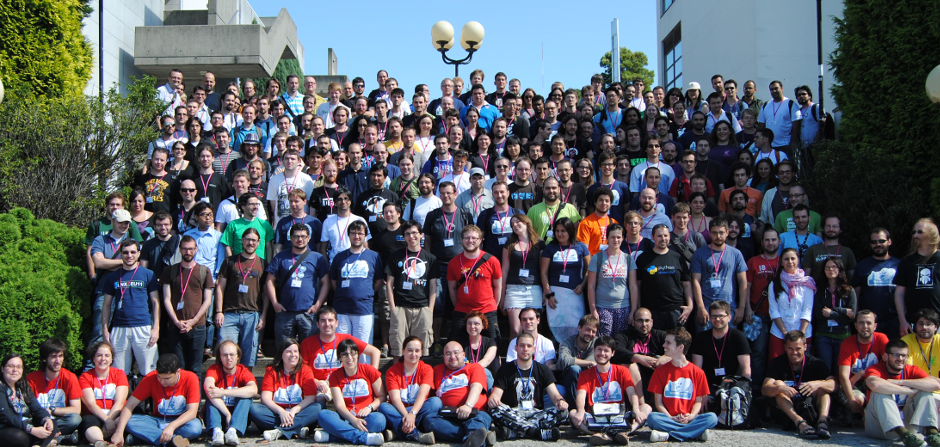
\includegraphics[width=\textwidth]{img/guadec_2012.png}
    \caption{GUADEC A Coruña 2012}
    \label{fig:guadec2012}
\end{figure}

Como comunidade reúne a gran cantidade de persoas tanto voluntarias como profesionais axudaron e axudan a que o proxecto siga adiante. Dentro desta comunidade poden encontrarse persoas de moi diversa procedencia e oficio sendo a maioría programadores aínda que tamén existen persoas dedicadas a marketing, administración, deseño, administración de sistemas, entre outras.

GNOME ademais pon especial interés en intentar sumar xente ao proxecto participando sempre no programa de iniciación ao desenvolvemento de software libre Summer of Code promovido por Google e sendo promotor da iniciativa Outreachy\footnote{Inicialmente denominábase GNOME Outreach Program for Women} que pretende acercar as mulleres á contribución en software libre.

En Europa a comunidade de GNOME reunese na GUADEC, que é o acrónimo de \textbf{G}NOME \textbf{U}sers \textbf{A}nd \textbf{D}evelopers \textbf{C}onference. Un evento que se fai anualmente e que no ano 2012 tivo lugar na Facultade de Informatica da Coruña.

\subsection{Localización e Internacionalización no Proxecto GNOME}
Como xa dixemos un dos aspectos máis importante para o proxecto GNOME é o acercamento as persoas e para lograr isto ponse pleno interés na internacionalización e na localización do ambiente de escritorio e das aplicacións de GNOME. GNOME está traducido a máis de 50 idiomas moitos dos cales teñen máis do 90\% das cadeas traducidas.

O proxecto GNOME emprega o sistema GNU Gettext para internacionalizar e localizar os seus programas e conta con unha plataforma web de nome Damned Lies para xestionar a localización de todo o proxecto. Este programa amosa as estatísticas do estado actual das traducións e axuda a xestionar o ciclo de traballo dos tradutores. Permite asignar módulos a tradutores, que os tradutores suban os ficheiros traducidos e que se faga unha revisión do traballo do tradutor.

Outros proxectos de software como Facebook, Twitter ou, dentro do software libre, Ubuntu e Fedora contan con plataformas online dende as que se pode facer directamente a tradución. GNOME opta por facer a tradución \emph{offline} para que esta sexa dunha maior calidade.

Para que os tradutores poidan traballar de forma cómoda é necesario a existencia de ferramentas que lle faciliten o traballo. Estas ferramentas coñécense como CAT, que é o acrónimo de Computer Assisted Translation. Neste traballo preténdese realizar unha destas ferramentas centrada no proxecto GNOME.

\section{Motivación}
Durante a GUADEC Hispana\footnote{A GUADEC Hispana é a versión para castelanofalantes da GUADEC} 2012 que tivo lugar en A Coruña dentro da GUADEC do mesmo ano, asistín a unha charla impartida por Daniel Mustieles, o coordinador do equipo de tradutores ao castelán do proxecto GNOME. Nesta charla Daniel, resaltaba a necesidade de que o programa actual de asistencia a tradución fose mellorado. GTranslator está escrito en C e emprega unha biblioteca chamada GObject para facer orientación a obxectos dentro de C. Isto fai que achegarse o proxecto sexa complicado para un novato polo que falando con outros desenroladores da plataforma decidiuse que era mellor reescribir o programa noutra linguaxe e ao mesmo tempo arreglar algúns erros que tiña anteriormente o programa. Durante o ano seguinte presentei un proxecto para o Google Summer of Code para escribir un novo programa CAT para a plataforma GNOME. Este programa sería unha re-escritura e re-deseño de GTranslator nunha linguaxe de programación moito máis amigable, Vala.

\section{Estrutura da memoria}

A memoria componse de oito capítulos nos que se expón os pasos que se deron para crear o programa GNOMECAT.


\paragraph*{Capítulo 1. Introdución.}
Este capítulo.

\paragraph*{Capítulo 2. Estado do Arte.}
Neste capítulo intentaremos explicar...

\paragraph*{Capítulo 3. Fundamentos Tecnolóxicos.}

\paragraph*{Capítulo 4. Metodoloxía}

\paragraph*{Capítulo 5. Planificación e Seguimento.}

\paragraph*{Capítulo 6. Análise de Requisitos.}

\paragraph*{Capítulo 7. Desenrolo.}

\paragraph*{Capítulo 8. Testing.}

\paragraph*{Capítulo 9. Conclusións e Traballo Futuro.}






        \chapter[Estado do arte]{Estado do Arte\label{estado_do_arte}}

Neste capítulo explicarase como funciona a internacionalización e localización con GNU Gettext. Ademais analizaremos as diferentes alternativas que existen no mercado como ferramentas de asistencia a tradución e as características que cada unha incorpora. O final faremos un resumo das características que empregan os programas CAT\footnote{Computer Assisted Translation}.

\section{Internacionalización e localización con GNU Gettext}
Gettext é un sistema para a internacionalización e localización amplamente usado en entornos UNIX. Conta con varías implementacións, sendo a primeira de Sun Microsystems no ano 1990. A implementación máis usada é a que GNU liberou no ano 1995. Pese ser unha solución antiga, é a día de hoxe a mellor que se pode atopar no mercado.

Para internacionalizar un programa con GNU Gettext non empregaremos as cadeas de texto directamente como podería ser no seguinte programa de exemplo:

\begin{lstlisting}[language=C,label=some-code,caption=helloworld.c (Sen Internacionalizar)]
#include <stdio.h>

int
main ()
{
    printf ("Hello World!");
}
\end{lstlisting}

En lugar diso chamaremos a unha función especial que proporciona Gettext de nome \lstinline{gettext()} pero que é máis empregada a través do seu alias \lstinline{_()}. Ademais configuraremos o programa para que colla a tradución do idioma que queiramos. Desta forma o programa anterior quedaría:

\begin{lstlisting}[language=C,label=some-code,caption=helloworld.c]
#include <stdio.h>
#include <locale.h>
#include <libintl.h>

#define _(str) gettext(str)

#define

int
main ()
{
    setlocale (LC_ALL, "");
    bindtextdomain ("helloworld", "/usr/local/share/locale");
    textdomain ("helloworld");

    printf (_("Hello World!"));
}
\end{lstlisting}

A función \lstinline{gettext()} é a encargada de substituír a cadea orixinal pola tradución. Non obstante vemos que debemos configurar algunhas cousas antes de poder chamar á función.

En primeiro lugar debemos establecer a linguaxe que queremos empregar no programa. Para iso usamos a función \lstinline{setlocale()}. O primeiro argumento da función determina que parte do locale actual queremos modificar. Entre outras podemos atopar:

\begin{itemize}
    \item \textbf{LC\_ALL.} Queremos cambiar todo.
    \item \textbf{LC\_ADDRESS.} Queremos cambiar a forma de formatar os enderezos.
    \item \textbf{LC\_MESSAGES.} Os mensaxes do programa.
    \item \textbf{LC\_NUMERIC.} O formatado das cantidades non monetarias
    \item \textbf{LC\_TIME.} O formatado de datas e horas.
\end{itemize}

Por último especificamos o código de idioma ou no caso de empregar a cadea baleira empregamos os valores das variables de entorno.

Os códigos de idioma empregan a normativa ISO 639 polo que son da forma $$language[\_territory][.codeset][@modifier]$$ Por exemplo o código do galego empregando codificación UTF-8 é \lstinline{gl\_ES.UTF-8}.

Ademais debemos indicarlle o programa onde ten que atopar as traducións. Para iso empregamos a función \lstinline{bindtextdomain()} que liga un nome de dominio a unha ruta dentro do sistema e a función \lstinline{textdomain()} que lle indica o programa cal é o nome de dominio que debe empregar. Un dominio é un conxunto de cadeas que se empregan nunha parte determinada dun programa. Cada dominio debe ter un nome de dominio único dentro dun programa.

Con estes parámetros Gettext xa é capaz de atopar as traducións que no caso do programa anterior atoparíanse en \emph{/usr/local/share/locale/gl/LC\_MESSAGES/helloworld.mo}.

Unha vez que internacionalizamos o nosos programa debemos traducir as cadeas. Pero para traducir as cadeas debemos extraelas antes do código fonte. Para iso empregaremos a utilidade \emph{xgettext}. Empregando as opcións adecuadas obtemos o seguinte ficheiro:

\begin{lstlisting}[label=some-code,caption=helloworld.pot]
# SOME DESCRIPTIVE TITLE.
# Copyright (C) YEAR THE PACKAGE'S COPYRIGHT HOLDER
# This file is distributed under the same license as the PACKAGE package.
# FIRST AUTHOR <EMAIL@ADDRESS>, YEAR.
#
#, fuzzy
msgid ""
msgstr ""
"Project-Id-Version: PACKAGE VERSION\n"
"Report-Msgid-Bugs-To: \n"
"POT-Creation-Date: 2014-11-12 19:24+0100\n"
"PO-Revision-Date: YEAR-MO-DA HO:MI+ZONE\n"
"Last-Translator: FULL NAME <EMAIL@ADDRESS>\n"
"Language-Team: LANGUAGE <LL@li.org>\n"
"Language: \n"
"MIME-Version: 1.0\n"
"Content-Type: text/plain; charset=CHARSET\n"
"Content-Transfer-Encoding: 8bit\n"

#: helloworld.c:14
#, c-format
msgid "Hello World!"
msgstr ""
\end{lstlisting}

Os ficheiros Gettext coa estensión \emph{POT} trátanse de plantillas xenéricas para todos os idiomas. Para obter o arquivo especifico para o noso idioma debemos empregar a ferramenta \emph{msginit} coa que obteremos un ficheiro similar a este:

\begin{lstlisting}[label=some-code,caption=helloworld.po (Sen Traducir)]
# Galician translations for HELLOWORLD package.
# Copyright (C) 2014 THE HELLOWORLD COPYRIGHT HOLDER
# This file is distributed under the same license as the ch package.
# Marcos Chavarría Teijeiro <chavarria1991@gmail.com>, 2014.
#
msgid ""
msgstr ""
"Project-Id-Version: ch 01\n"
"Report-Msgid-Bugs-To: \n"
"POT-Creation-Date: 2014-11-12 19:24+0100\n"
"PO-Revision-Date: 2014-11-12 19:54+0100\n"
"Last-Translator: Marcos Chavarría Teijeiro <chavarria1991@gmail.com>\n"
"Language-Team: Galician\n"
"Language: gl_ES\n"
"MIME-Version: 1.0\n"
"Content-Type: text/plain; charset=ISO-8859-1\n"
"Content-Transfer-Encoding: 8bit\n"

#: helloworld.c:14
#, c-format
msgid "Hello World!"
msgstr ""
\end{lstlisting}

Desta forma obtemos un ficheiro Gettext PO que é o ficheiro que temos que editar. Traducindo o arquivo obtemos algo como isto:

\begin{lstlisting}[label=lst:translated_example,caption=helloworld.po (Traducido)]
# Galician translations for HELLOWORLD package.
# Copyright (C) 2014 THE HELLOWORLD COPYRIGHT HOLDER
# This file is distributed under the same license as the HELLOWORLD package.
# Marcos Chavarría Teijeiro <chavarria1991@gmail.com>, 2014.
#
msgid ""
msgstr ""
"Project-Id-Version: HELLOWORLD 1.0\n"
"Report-Msgid-Bugs-To: \n"
"POT-Creation-Date: 2014-11-12 19:24+0100\n"
"PO-Revision-Date: 2014-11-12 19:54+0100\n"
"Last-Translator: Marcos Chavarría Teijeiro <chavarria1991@gmail.com>\n"
"Language-Team: Galician\n"
"Language: gl_ES\n"
"MIME-Version: 1.0\n"
"Content-Type: text/plain; charset=ISO-8859-1\n"
"Content-Transfer-Encoding: 8bit\n"

#: helloworld.c:14
#, c-format
msgid "Hello World!"
msgstr "Ola Mundo!"
\end{lstlisting}

Antes de poder empregar o ficheiro no noso programa temos que compilalo. Para iso empregamos a utilidade msgfmt ca que obtemos o ficheiro helloworld.mo. Se movemos o ficheiro o directorio adecuado (o que especificamos en \lstinline{textdomain()}) o noso programa xa estará localizado.

%http://www.gnu.org/software/libc/manual/html_node/Locating-gettext-catalog.html

\subsection{Ficheiros Gettext PO}
Como xa dixemos antes os ficheiros PO son os ficheiros que temos que editar para localizar o noso programa. Primeiro dicir que se trata ficheiros de texto plano e que polo tanto podemos editar con calquera editor de ficheiros de texto plano. Non obstante, o ideal é empregar algunha ferramenta que nos facilite a tarefa como pode ser unha ferramenta CAT.

As súas principais características son:

\paragraph{Soporte de plurais}
Algo que pode parecer trivial como o soporte de plurais deixa de selo cando consideramos que non todos as linguaxes do mundo empregan dous plurais. A lingua eslovaca, por exemplo, conta con tres formas de plural de forma que o plural faise diferente para 1, 3 e 5 elementos.

Gettext representa a forma de plural de cada linguaxe con unha cadea da seguinte forma: $$nplurals=n; plural=exp;$$ Onde $n$ representa o número de plurais da linguaxe e $exp$ a expresión para calcular cando debemos empregar cada forma. Por exemplo a forma plural do galego representase como $nplurals=2; plural=(n != 1);$. Isto é que temos 2 plurais e que so se emprega a forma singular cando o número de elementos é igual a $1$.

No código fonte para que GetText escolla a tradución adecuada temos que empregar a función \lstinline{ngettext}. Esta función recibe como parámetros a cadea orixinal en singular, a cadea orixinal en plural e o número de elementos. No seguinte fragmento de código temos un exemplo:

\begin{lstlisting}[language=C,caption=Plurais en GetText (Código Fonte).]
[...]
    printf (ngettext ("We have %d car.", "We have %d cars.", n), n);
[...]
\end{lstlisting}

A cadea do ficheiro PO correspondente o código anterior pódese ver no seguinte fragmento de código. Vemos como temos unha entrada \lstinline{msgstr} por cada plural. Desta forma o plural número $0$ corresponde os singular é o plural número $1$ correspondese coa primeira forma do plural.

\begin{lstlisting}[caption=Plurais en GetText (Ficheiro PO).]
#: helloworld.c:19
#, c-format
msgid "We have %d car."
msgid_plural "We have %d cars."
msgstr[0] "Temos %d coche."
msgstr[1] "Temos %d coches."
\end{lstlisting}


\paragraph {Marcado de traducións difusas}
Permítese marcar certas traducións como difusas de forma que o tradutor indica que non estar seguro de que dita tradución sexa correcta. Se marcásemos a tradución \emph{"Hello World!"} como difusa o ficheiro PO tería o seguinte aspecto:

\begin{lstlisting}[label=some-code,caption=Ficheiro POT con comentario.]
[...]
#: helloworld.c:15
#, c-format
#, fuzzy
msgid "Hello World!"
msgstr ""
[...]
\end{lstlisting}

\paragraph {Formato das traducións}
Os ficheiro PO permite indicar se as cadeas a traducir teñen un formato determinado. Por exemplo a cadea do exemplo no Fragmento de Código \ref{lst:translated_example} pódese ver que ten o flag \lstinline{c-format} debido a que é parte dunha sentencia printf e podería levar indicadores de formato da forma \lstinline{%s}.

\paragraph {Cabeceira con metadatos}
Existe unha cadea especial nos documentos Gettext PO. Trátase da cadea baleira que serve para almacenar metadatos do ficheiro. No fragmento de código \ref{lst:translated_example} podemos ver istos metadatos. Algúns dos metadatos existentes son:

\begin{itemize}
    \item \textbf{Project-Id-Version.} Nome único para o proxecto deste arquivo de tradución.
    \item \textbf{Report-Msgid-Bugs-To.} Ligazón onde reportar errores nas cadeas orixinais ou para pedir contexto para facer a tradución.
    \item \textbf{POT-Creation-Date.} Data de creación do ficheiro POT.
    \item \textbf{PO-Revision-Date.} Data da última actualización das traducións.
    \item \textbf{Last-Translator.} Nome e enderezo de correo electronico do último traductor.
    \item \textbf{Language-Team.} Enderezo de correo eléctronico do equipo de traductores.
    \item \textbf{Language.} Linguaxe do ficheiro expresada coa codificación ISO 639.
    \item \textbf{Content-Type.} Tipo MIME do ficheiro, que será sempre \lstinline{text/plain} e codificación dos caracteres.
    \item \textbf{Plural-Forms.} Expresión da forma plural empregada.
\end{itemize}

Ademais destes campos, nos comentarios, gárdanse os nomes de todas as persoas que contribuíron a esta tradución.

\paragraph{Gardado dos orixes das cadeas}
Gettext almacena para cada cadea en que lugares do código aparece esta. O cal pode ser moi interesante para implentar a previsualización das traducións. Por exemplo no Fragmento de Código~\ref{lst:translated_example} vemos como a cadea \emph{"Hello World!"} pode atoparse na liña 14 do ficheiro \lstinline{helloworld.c}.

\paragraph{Comentarios dos programadores}
É unha función moi importante xa que en moitas ocasións nas linguaxes a mesma palabra empregase como verbo ou como nome polo que en ocasións é importante incorporar un contexto para esa tradución. Para facer isto é necesario simplemente poñer un comentario no programa antes de empregar a cadea. Por exemplo no seguinte fragmento de código:

\begin{lstlisting}[language=C,caption=Tradución con comentario.]
[...]
    // Translators: We are just waving the world.
    printf (_("Hello World!"));
[...]
\end{lstlisting}

Estamos engadindo un comentario a cadea \emph{"Hello World!"}. O ficheiro POT resultado tería a forma:

\begin{lstlisting}[label=some-code,caption=Ficheiro POT con comentario.]
[...]
#. Translators: We are just waving the world.
#: helloworld.c:15
#, c-format
msgid "Hello World!"
msgstr ""
[...]
\end{lstlisting}


\paragraph{Comentarios dos tradutores}
A biblioteca permite que os tradutores comenten as cadeas. Engadindo un comentario á cadea \emph{"Hello World!"}, o ficheiro PO tería o seguinte aspecto:

\begin{lstlisting}[caption=Ficheiro PO con comentario.]
[...]
# This is a note from translators.
#: helloworld.c:15
#, c-format
msgid "Hello World!"
msgstr ""
[...]
\end{lstlisting}

\section{Ferramentas CAT do mercado}
\label{sec:ferramentascat}
Nesta sección analizaremos algunhas das ferramentas de asistencia a tradución existentes. Veremos as características que incorporan estes programas así como estudar a súa interface de usuario.

\subsection{GTranslator}
GTranslator é a aplicación oficial do proxecto GNOME para a asistencia a tradución. Este aplicativo so permite a tradución de arquivos GNU Gettext. As característica máis destacables deste programa son a posibilidade de abrir varios ficheiros en diferentes lapelas, soporte de memorias de tradución, perfiles para diferentes tradutores, edición dos comentarios dos ficheiros .po e un sistema de plugins que permite estender a ferramenta.

\begin{figure}[h]
    \centering
    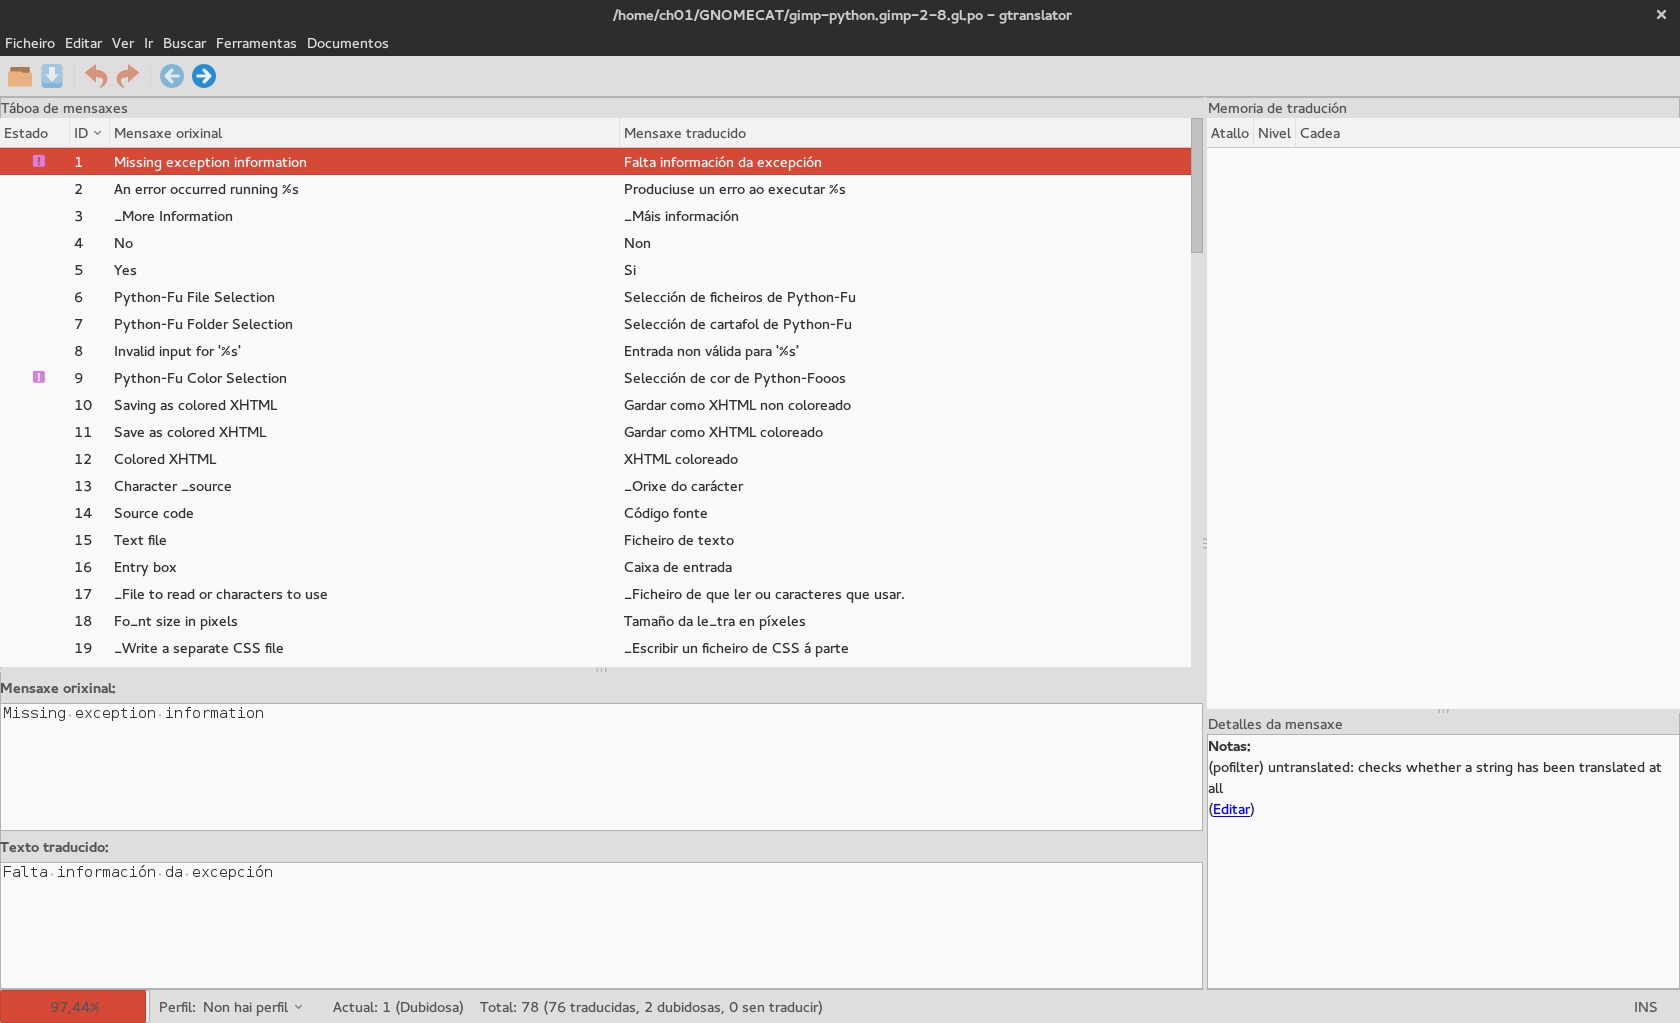
\includegraphics[width=\textwidth]{img/captura_gtranslator.png}
    \caption[Interface de GTranslator]{Interface de GTranslator}
    \label{fig:gtranslator}
\end{figure}

En canto a interface, como podemos ver na Figura~\ref{fig:gtranslator}, a parte máis importante do programa é a a lista de mensaxes. Abaixo desta lista temos un panel onde se pode editar cada mensaxe e a súa dereita a memoria de tradución. A disposición dos elementos desta interface é configurable xa que permite mover e ampliar cada un dos módulos. O programa tamén incorpora atallos de teclado que permiten moverse polo documento e seleccionar cada elemento da memoria de tradución.

Este programa pese a ser o aplicativo oficial de GNOME é moi pouco usado. As razóns disto son a ausencia dunha característica chave que o diferencie doutras ferramentas do mercado, a presencia de fallas importantes que afectan a usabilidade e a ausencia dun mantedor que resolva estes problemas.

\subsection{Lokalize}
Lokalize é o programa oficial para o soporte a tradución en KDE. Foi escrita dende cero empregando a tecnoloxía de KDE Platform 4 e baseándose no código de KBabel. As súas características máis destacables son, o soporte para ficheros GNU Gettext e o formato QT TS entre outros; a xestión de proxectos incorporando unha vista que permite ver un resumo de cada ficheiro dentro do proxecto; uso de memorias de tradución e de glosarios; comprobación da ortografía e vista previa das traducións a partir de scripts feitos polo usuario.

\begin{figure}[h]
    \centering
    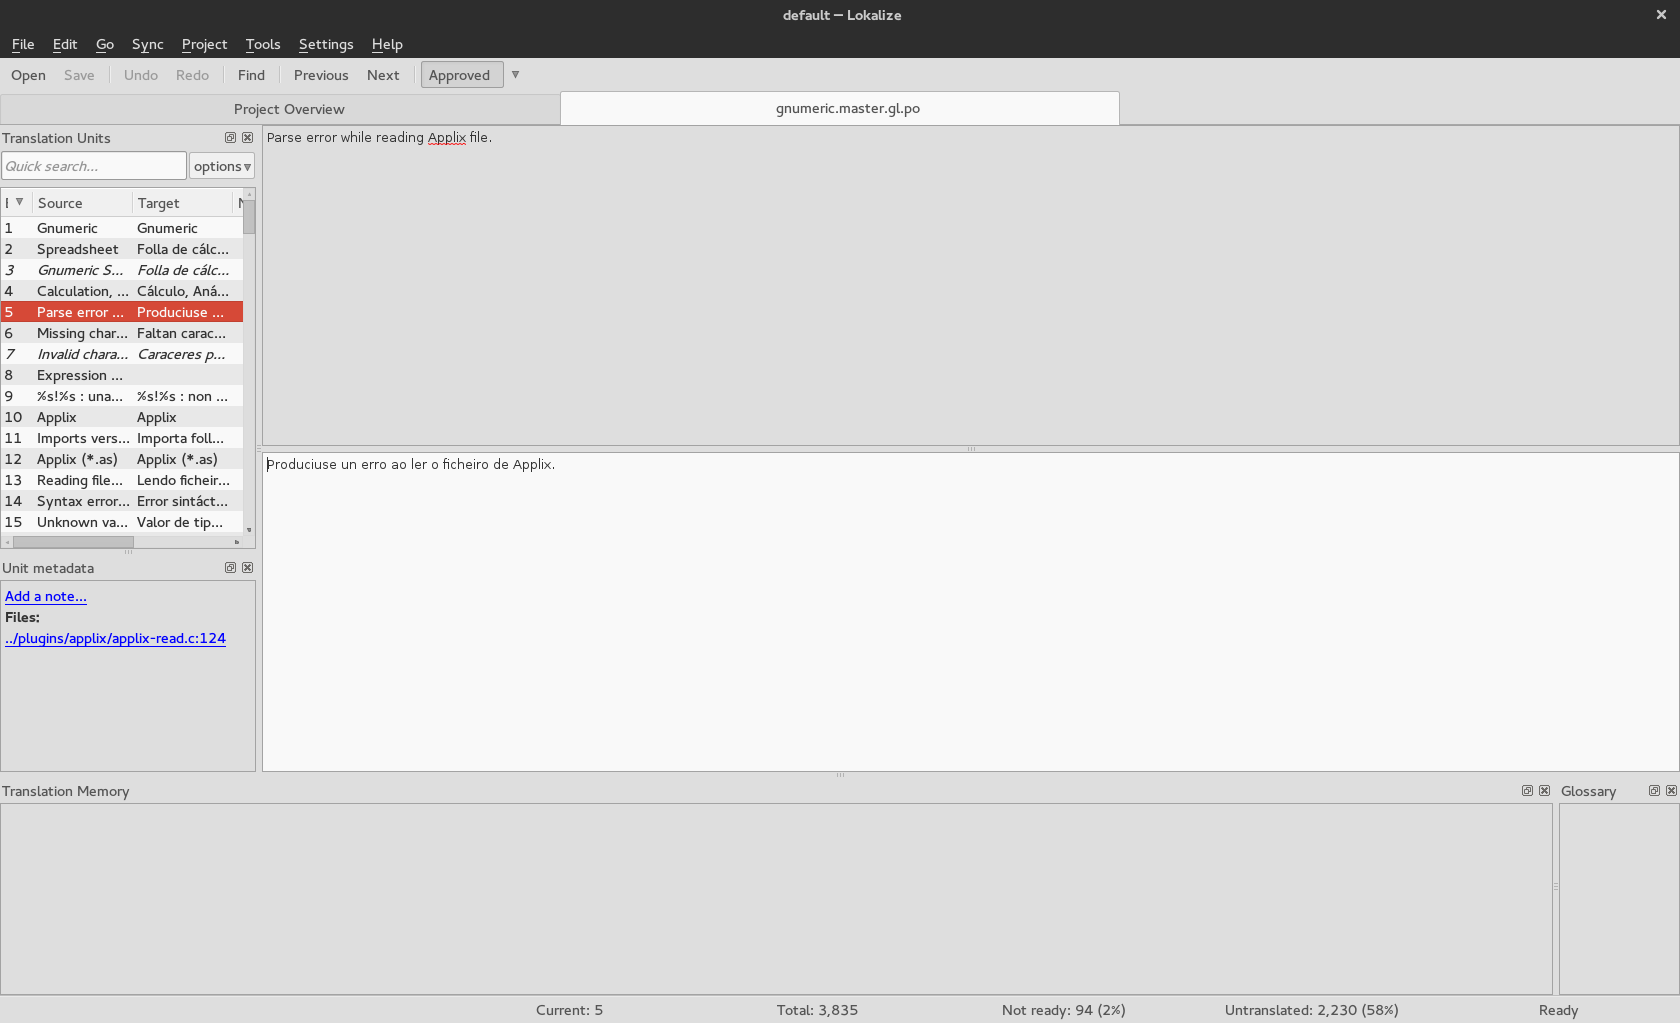
\includegraphics[width=\textwidth]{img/captura_lokalize.png}
    \caption{Interface de Lokalize}
    \label{fig:lokalize}
\end{figure}

En canto a interface, o programa permite abrir varios ficheiros cada un na súa lapela. Como se pode ver na Figura~\ref{fig:lokalize}, a vista de tradución está centrada no panel de edición, onde aparecen tanto a cadea orixinal como a cadea a traducir. Na columna da esquerda podemos ver a lista de cadeas onde se amosan os primeiros caracteres da cadea orixinal e da tradución e o estado desta tradución. Ademais tamén se pode ver o contexto da tradución, engadir un novo comentario e ver en que ficheiros estaba dita tradución. Por último tamén podemos ver na parte inferior a memoria de tradución e o glosario.

\subsection{Virtaal}

Virtaal é unha ferramenta CAT creada por Translate House\footnote{Compañía que surxiu a partir dunha comunidade de tradutores de Sudáfrica e que está especializada na creación de ferramentas e bibliotecas para axudar a tradución.} As características máis destacables son a incorporación de suxestión a tradución, comprobación da calidade das tradución e, sobretodo, a capacidade de abrir unha gran variedade de formatos a través da biblioteca Translate Toolkit.

\begin{figure}[h]
    \centering
    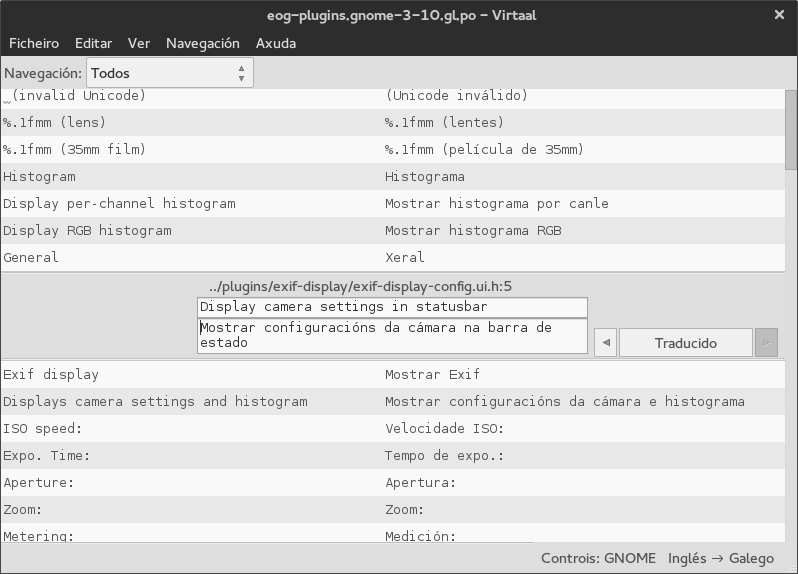
\includegraphics[width=\textwidth]{img/captura_virtaal.png}
    \caption{Interface de Virtaal}
    \label{fig:virtaal}
\end{figure}

Como se pode ver na Figura~\ref{fig:virtaal}, a interface é minimalista e moi centrada na tradución. A diferencia dos casos anteriores, trátase dunha interface fixa e que integra a lista das mensaxes coa edición da propia mensaxe. Tamén se indican posibles fallos que poidan ter a tradución, como falta de puntos o final, ausencia de marcadores de formato, etc.

\subsection{OmegaT}
Ferramenta CAT lanzada no ano 2001 e pensada fundamentalmente para tradutores profesionais. Ten soporte para o uso de memoria de tradución, glosario, tradución directa entre outras cousas. Destaca a gran cantidade de formatos que pode empregar.

\begin{figure}[h]
    \centering
    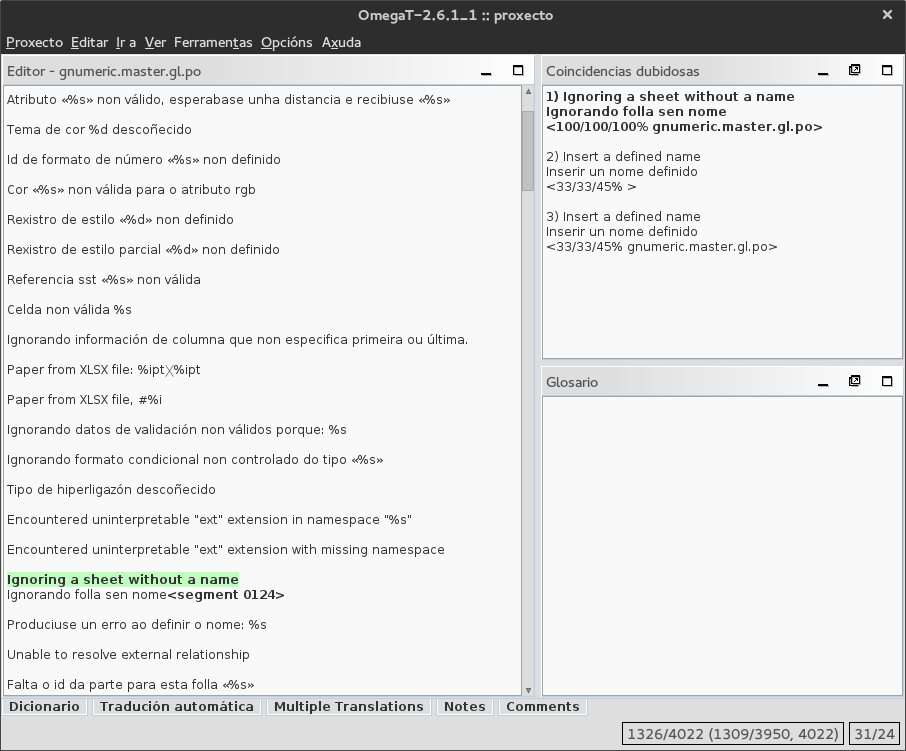
\includegraphics[width=\textwidth]{img/captura_omegat.png}
    \caption{Interface de OmegaT}
    \label{fig:omegat}
\end{figure}

A interface de OmegaT dista bastante do resto de programas. Como amosa a Figura~\ref{fig:omegat} non existe o concepto de lista de mensaxes traducir. O documento amosase como unha sucesión de cadea e se facemos clic encima dunha, permitiranos traducila. Trátase dun programa moi usado para a tradución tanto profesional como amateur.

\subsection{Google Translation Toolkit}
É a ferramenta CAT desenvolvida por Google e lanzada no ano 2008. A diferencia dos aplicativos analizados anteriormente, esta trátase unha solución puramente web. Entre as súas principais características encontrase a posibilidade de facer tradución automática empregando Google Translator, o uso de memorias de tradución compartidas, glosarios, soporte de etiquetas HTML entre outros e atallos de teclado. Ten soporte para varios formatos como ficheiros PO, documentos de Microsoft Word, de LibreOffice ou mesmo artigos da Wikipedia.

\begin{figure}[h]
    \centering
    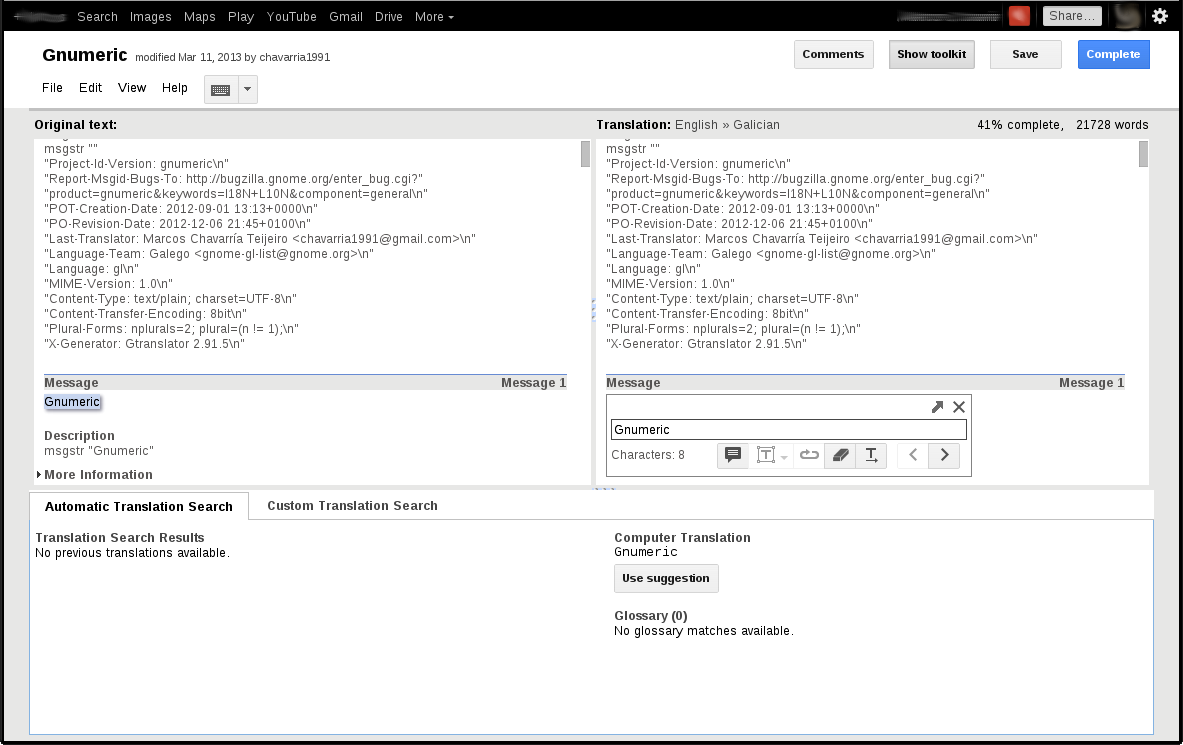
\includegraphics[width=\textwidth]{img/captura_googletranslationtoolkit.png}
    \caption{Interface de Google Translation Toolkit}
    \label{fig:translatetoolkit}
\end{figure}

Como se pode ver na Figura~\ref{fig:translatetoolkit}, na interface misturase a lista de cadeas co cadro de edición das mesmas. Ademais empregando unha interface semellante a do resto de ferramentas ofimáticas de Google, temos botóns para autocompletar tags e para avanzar a seguinte tradución. Aínda que foi pensado para a tradución colaborativa de documentos de ONGs e artigos da Wikipedia, na actualidade emprégase maioritariamente para a tradución de proxectos comerciais.


\subsection{Transifex}
Trátase dunha plataforma que xurdiu a partir dun proxecto do Google Summer of Code do ano 2007 que pretendía crear unha plataforma online máis amigable que o Damned Lies de GNOME que naquel momento tamén empregaba Fedora unha distribución de GNU/Linux. Trátase dunha solución de pago con plans que van dende os 19 a os 300 dólares. Non obstante os proxectos de código aberto poden usar o servizo de forma gratuíta e dispón de un período de mostra 30 días. As súas principais características son a posibilidade de descargar o documento e volvelo a subir para poder traducilo con outra ferramenta CAT, editor online, memoria de tradución e unha API que permite integralo con outros servizos. Ademais tamén soporta unha gran variedade de formatos entre os que se atopan os ficheiros PO, DTD de Mozilla ou XML entre outros.

\begin{figure}[h]
    \centering
    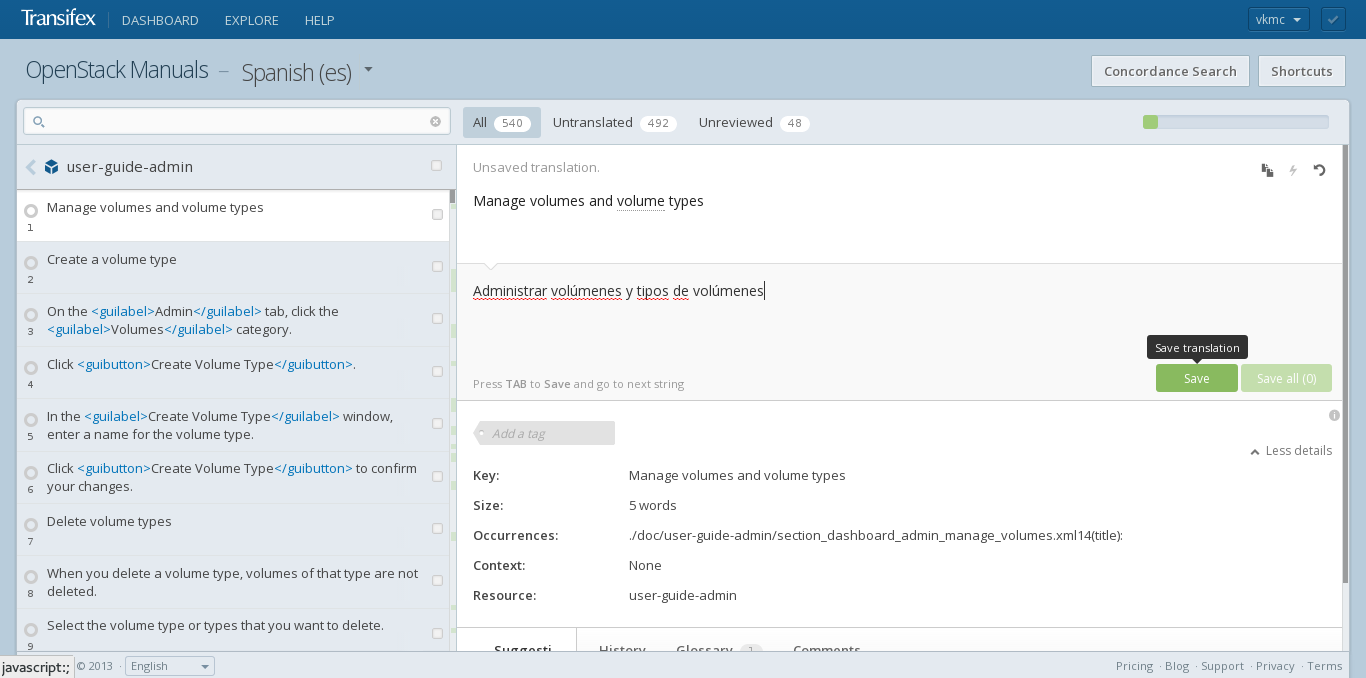
\includegraphics[width=\textwidth]{img/captura_transifex.png}
    \caption{Interface de Transifex}
    \label{fig:transifex}
\end{figure}

A interface de trasifex, como ser pode ver na Figura~\ref{fig:transifex} separa a lista de cadeas do cadro de edición. No cadro de edición temos a posibilidade de consultar a memoria de tradución ou o glosario. O programa tamén incorpora resaltado de sintaxe.

\subsection{Outras ferramentas}
Existen moitas máis ferramentas CAT no mercado. De feito, segundo unha enquisa \cite{article:2006survey} elaborada polo Imperial College London a cerca de 900 tradutores profesionais de 54 países diferentes, os únicos programas de todos os anteriores que aparecen citados é o OmegaT que conta con un 7\% de usuarios. As ferramentas máis usadas son ferramentas para Microsoft Windows e ferramentas con licencias privativas e usualmente moi caras. Algunhas destas ferramentas son TRADOS, Wordfast, DejaVu SDLX ou STAR Transit. Na Figura~\ref{fig:enquisa2006} podemos ver unha gráfica coas ferramentas máis empregadas segundo este estudio.

\begin{figure}[h]
    \centering
    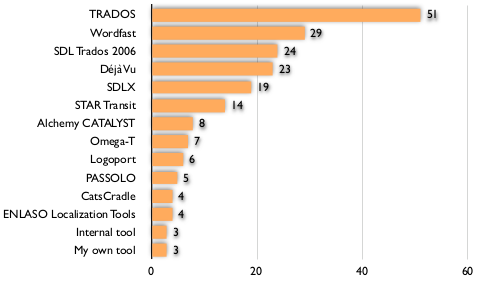
\includegraphics[width=0.7\textwidth]{img/grafico_uso_cat_enquisa2006.png}
    \caption{Ferramentas CAT máis empregadas segundo \cite{article:2006survey}.}
    \label{fig:enquisa2006}
\end{figure}

Hai que ter tamén en conta que se trata dun estudio bastante antigo polo que algunhas das ferramentas analizadas aínda non existían. Por exemplo a enquisa cita a ferramenta KBabel, que é a ferramenta de KDE na que está baseada Lokalize, pero con menos dun 2\% de usuarios.


\section{Características xenéricas das ferramentas CAT}

Algunhas das características que aparecen de forma recurrente en todas as ferramentas analizadas son as seguintes:

\subsection{Memoria de Tradución}
Unha memoria de tradución é unha base de datos composta de textos orixinais acompañados das súas traducións. Estes textos almacénanse en segmentos onde a separación entre segmentos ven dada por signos de puntuación ou o cambio de parágrafo, sendo esta última forma a máis frecuente.

A principal función dunha memoria de tradución e a extracción de coincidencias totais ou parciais. Os programas que teñen esta característica buscan na base de datos un segmento que coincida de forma exacta ou parcial coa cadea que se está a traducir e mostrase este segmento como suxerencia. Xunto coa suxerencia tamén se amosa o grado de cercanía entre a cadea a traducir e a cadea da memoria de tradución.

Existe un formato estándar de compartición de memorias de tradución de nome Translation Memory eXchange (TMX) e plataformas online que almacenan gran cantidade de cadeas e polo tanto hai máis posibilidade de obter unha mellor coincidencia. O software Amagama creado por Translate House, os creadores de Virtal, é un exemplo de memoria de tradución online.

\subsection{Glosario}
Un glosario é unha base de datos de termos xunto con unha ou varias traducións aceptadas. Diferenciase da memoria de tradución en que so se proporcionan a tradución a termos e non a cadeas completas. De igual forma que no caso das memorias de tradución, existe un formato estándar de para a compartición de glosarios de nome TermBase eXchange (TBX) e plataformas online para almacenar os glosarios.


\subsection{Previsualización}
As funcións de previsualización permítenlle ó tradutor ver como vai quedar a cadea traducida no programa final.

Os programadores e deseñadores fan as interfaces tendo en conta a lingua orixinal e non ningunha das traducións polo que se unha tradución é moito máis longa ca orixinal pode verse mal no programa final.

Para conseguir esta característica pódense empregar varias técnicas:

\begin{itemize}
  \item \textbf{Programa orixinal.} Esta técnica que se pode empregar en calquera cadea consiste en compilar o ficheiro PO e executar o programa final con ese ficheiro PO. Desta poderemos ver como queda a nosa tradución para o usuario final. A desvantaxe deste método consiste en que teremos que saber en que parte do programa se emprega a cadea que queremos previsualizar. Este método é empregado por Lokalize que permite a definición de scripts para a previsualización de cadeas.

  \item \textbf{Renderizado de interfaces de usuario en XML.} Nas bibliotecas de interfaces modernas existe a posibilidade de definir interfaces en ficheiros XML e despois renderizalas. Neste caso as cadeas a traducir van nestes arquivos e sería posible renderizar esta interface coa tradución que estamos a realizar. Este método aínda que si que amosaría a pantalla onde aparece a cadea actual, so é válido para as cadeas que proveñen destes ficheiros XML e non as definidas da forma tradicional. Un exemplo deste método pódese ver na rede no aplicativo Deckard\footnote{\href{http://deckard.malizor.org/}{deckard.malizor.org}} que permite ver as traducións de aplicativos de GNOME.
\end{itemize}


\subsection{Tradución Directa}
A tradución de cadeas de forma automática empregando algoritmos deseñados a tal proceso e que empregan grandes bases de datos aloxadas, xeralmente en internet. Tanto Google como Microsoft teñen os seus produtos corporativos que fan traducións e existen alternativas libres como OpenTrad ou Apertium. Estas traducións aínda que validas soen ser de baixa calidade polo que necesitan unha revisión.

        \chapter{Fundamentos Tecnolóxicos}

\section{Ferramentas empregadas}

\paragraph{Vala} É unha linguaxe de programación orientada a obxectos creada por GNOME para acercar a linguaxe de programación C as caracteristicas das linguaxes de programación modernas. Emprega a linguaxe de programación C xunto coa biblioteca GObject como linguaxe intermedio. Esta linguaxe cunha sintaxe moi parecida a C\# incorpora caracteristicas como o uso e funcións anónimas, bucles foreach, xestión automatica de memoria ou o manexo de excepcións.

Tradicionalmente a linguaxe oficial de GNOME era C. Esta linguaxe moi empregada en moitos proxectos de software libre como pode ser o kernel de Linux carece sen embargo de caracteristicas propias da orientación a obxetos. A librería GObject, aínda que fornece á linguaxe destas caracteristica, é tremendamente verbosa e moi complexa para os principiantes.

Escolleuse esta linguaxe por ter unha sintaxe moi amigable, o que pode axudar a que programadores con pouca experiencia se interesen polo proxecto e por incorporar certa integración con algunhas librerías de GNOME que fai que o código final sexa moito máis limpo.

 \paragraph{Autotools} Tamén coñecidas como \emph{GNU build system} son un conxunto de ferramentas que permiten permitir a creación e compilación de programas portables a varias plataformas UNIX.

 \paragraph{Git} É un sistema de control de versións distribuido escrito por Linux Torbards e usado, entre outros moitos proxectos, para xestionar o desenrolo de Linux (o kernel).

Escolleuse esta opción por permitir traballar en local, por ser moi rápido e por ser o sistema de control de versións moderno máis empregado actualmente.

 \paragraph{GitHub} Unha plataforma de almacenamento de proxectos empregando o sistema de control de versións Git. Permite subir proxectos Open Source de forma gratuita os seus servidores. Ademais de permitir subir os ficheiros ten ferramentas para a creación de Wikis relacionadas cos proxectos e para a xestión de incidencias. Esta ferramenta para a xestión de incidencias for empregada para facer o seguimento do proxecto.

 \paragraph{Listas de Correo} As listas de correo son un medio de comunicación asíncrona moi usadas no mundo do desarrollo software. Os usuarios escriben un correo electronico a un enderezo especial que reenvia dito correo a todos os usuarios subscritos as listas. Ademais os correos enviados a lista son almacenados nun historial para a súa posterior consulta.


 \paragraph{IRC (Internet Relay Chat)} É un protocolo de comunicación entre usuarios creado no ano 1988. É amplamente usado no mundo do desarrollo software como unha ferramenta rápida para consultar dubidas entre desarrolladores. Existen multiples clientes dispoñibles para case calquera plataforma. En concreto empregouse o programa XChat.

 \paragraph{JHBuild} Unha serie de scripts que permiten a descarga automatica do código fonte dun proxecto e das súas dependencias e a instalación destes proxectos dentro dun entorno chroot. Desta forma os desarrolladores poden traballar coas últimas versións das bibliotecas que tenden a ser inestables sen ter que usalas en todo os seu sistema.

\paragraph{Glade} Unha ferramenta para a creación de interfaces de usuario con GTK+ as interfaces creadas exportanse en ficheiros con formato XML.

\paragraph{Dia} É un programa para a creación de diagramas de todo tipo. Ten un paquete para facer diagramas UML.

\paragraph{JSON} É un formato para o intercambio de datos. Acronimo de JavaScript Object Notation, trátase dun subconxunto da notación para definir obxectos en JavaScript. Para poder analizar este formato no noso programa empregaremos a biblioteca JSON-GLib.

\paragraph{GDB} GNU Project debugger. É o depurador estandar para o proxecto GNU. Permite a execución paso a paso, monitorizar e alterar o valor das variables entre outras moitas características.

\paragraph{\LaTeX}

\paragraph{DogTail}


\section{Bibliotecas empregadas}

\paragraph{GLib} É unha biblioteca de propósito xeral creada por GNOME a partir de 5 librerías, GObject, GLib, GModule, GThread e GIO.

\emph{GObject} incorpora características da orientación a obxectos a linguaxe de programación C, como pode ser a creación de clases, herencia ou as propiedades entre outras. \emph{GLib} constitue un conxuto de tipos básicos empregados no resto de bibliotecas. \emph{GModule} permite a carga de modulos ou extensións de forma dinamica. Por último, \emph{GThread} é unha biblioteca de xestión de fíos de execución e \emph{GIO} é unha biblioteca pensada para facilitar a entrada e saída nos programas.

Esta bibliotaca constitue unha dependencia básica en todas os aplicativos feitos co \emph{stack} de GNOME e, de feito, é unha dependencia de case todas as demais bibliotecas que empregamos.

\paragraph{GTK+} Biblioteca multiplataforma para a creación de interfaces gráficas de usuario desenvolvida por GNOME. Incorpora unha serie de widgets para a creación de programas tanto grandes como pequenos. Está escrita en C pero existen bindings para moitas linguaxes.

\lstinputlisting[language=C,label=lst:gtkcexample,caption=Exemplo de interface GTK+ en C]{examples/gtk_example.c}

As interfaces gráficas podense crear de forma programática (como se pode ver no Fragmento de Código~\ref{lst:gtkcexample}) ou cargando un ficheiro XML (como o que se mostra no Fragmento de Código~\ref{lst:gtkgladeexample}).

\lstinputlisting[language=XML,label=lst:gtkgladeexample,caption=Examplo de interface GTK+ en XML]{examples/glade_example.ui}

Aínda que pode parecer moito máis traballoso a creación dun ficheiro XML con ese propósito, a existencia de ferramentas como Glade\footnote{\href{http://glade.gnome.org}{glade.gnome.org}}.

\paragraph{LibGee} Trátase dunha biblioteca que fornece a GObject de estructuras de datos comunmente usadas como listas, tablas hash ou conxuntos entre outros.

\paragraph{LibPeas} LibPeas é un motor de plugins para GObject. Escrito orixinalmente para GEdit permite as aplicacións extenderse a través dun sistema de plugins.

\paragraph{GettextPo} Trátase dunha biblioteca que analiza ficheiros GNU Gettext PO. Esta biblioteca está implementada en C e non existen bindings para Vala polo que teremos que facelos nós.

\paragraph{GTKSourceView} Esta bibioteca extende o \emph{widget} de GTK+ GtkTextView, que permite a visualización de textos, para incorporarlle certas características avanzadas como a xestión de cambios permitindo desfacer e refacer ou o resaltado da sintaxe.

\paragraph{JSON-GLib} É unha biblioteca para a análise de cadeas de texto en formato JSON.

        \chapter{Metodoloxía}

Nesta sección descríbese a metodoloxía levada a cabo para a realización deste proxecto. Unha metodoloxía e un conxunto de métodos ou prácticas empregadas para a realización dunha tarefa, neste caso o analise, deseño e implementación dunha nova ferramenta CAT para o proxecto GNOME. Escolleuse unha metodoloxía axil de ciclo incremental. Moitas das prácticas que se tomaron son collidas da metodoloxía eXtreme Programming.

\section{eXtreme Programming}

Foi creada por Kent Beck no ano 1999 e trátase dun dos máis destacados métodos de desenvolvemento áxil. eXtreme Programming (a partir de agora XP) avoga por ciclos de desarrollo moi curtos e elimina os roles clásicos de analista, deseñador e programador. Todo equipo participa en todas as partes do desarrollo. Desta forma Beck define uns valores fundamentais da metodoloxía e unhas prácticas que axudan a adoptar estos valores.

\subsection{Valores de eXtreme Programming}

\subsubsection{Comunicación}
É o primeiro valor de XP. Segundo esta metodoloxía os problemas nos proxectos poden ser traducidos a alguén que non falou con outra persoa sobre algo importante do proxecto. Esta mala comunicación non sucede por casualidade e é debido frecuentemente as malas prácticas. Para solucionar isto, XP inclúe prácticas nas que é necesario a comunicación para levalas a cabo. Ademais a figura do \emph{coach} sirve para mellorar a comunicación daquelas persoas que non o están facendo ben.

\subsubsection{Simplicidade}

A simplicidade non é unha tarefa sinxela. XP fai unha aposta e invita ao programador a pensar no que o proxecto necesita hoxe e non no que vai necesitar nun futuro. Para manter esta simplicidade ao longo do tempo é frecuente a refactorización do mesmo para manter dita simplicidade. A simplificación do deseño e da implementación axiliza tanto o desenvolvemento como o mantemento. A simplicidade require \textbf{comunicación} pois canto máis comunicación teñamos por parte do cliente máis sinxelo simple poderemos facer o sistema e canto máis simple sexa o sistema menos comunicación será necesaria para explicar o sistema.

\subsubsection{Retroalimentación}
A retroalimentación ou feedback é fundamental nesta métodoloxía. Pode actuar en varias escalas de tempo. Obtemos feedback en cuestion de minutos ou días de parte dos test do sistema, das peticións dos clientes ou do director do proxecto. Tamen obtemos feedback o longo dos meses cando o usuario pode analizar as caracteristicas que implementamos. Neste sentido XP aposta por unha posta rápida en produción de forma que teñamos sistemas en produción e en desarrollo de forma paralela. Con isto melloramos o sistema xa que imos obtendo as opinións dos usuarios das decisións que xa tomamos e os erros cometidos non se volven a repetir.

\subsubsection{Coraxe}
O coraxe é unha parte inherente a metodoloxía. É necesario para tirar o traballo de varios días e volver e empezar debido a cambios nos requisitos ou aparición de fallos estructurais. É necesario para ser persistente ca resolución dun problema, as cousas que non se dan resolto un día en horas podense resolver o día seguinte en cuestión de minutos. O coraxe non é útil sen os tres primeiros valores. Con unha boa comunicación existe a posibilidade de facer experimentos con máis risco. A simplicidade permite o programador coñecer mellor o código e polo tanto ser máis valiente a hora de facer cambios. A retroalimentación axuda a que alguén se sinta máis seguro ao facer un cambio.

\subsubsection{Respeto}
Por último é necesario respeto. É necesario que os integrantes do equipo se preocupen polo resto de membros e polo que están facendo. Ademais o equipo debe preocuparse polo propio proxecto. Para que XP funcione os programadores debense sentir parte do proxecto e ter un feedback positivo ao respecto.

\subsection{Prácticas recomendadas por eXtreme Programming}

\subsubsection{O Xogo da Planificación}
A planificación é un dialogo entre a xente do negocio e o equipo técnico. Mentras a parte de negodio decide a importancia dun problema, aprioridade da implementación dunha característica ou outra, a composición das entregas ou as datas das mesmas, o equipo técnico é capaz de estimar canto tempo leva implementar unha característica, ten a capacidade de explicar as consecuencias de certa decisión, sabe como organizarse para levar a cabo unha tarefa e pode facer unha planificación máis detallada.

\subsubsection{Entregas Pequenas}
As entregas ou \emph{releases} deben ser o máis pequenas posibles e conter os requerimentos máis valiosos. Aínda así cada release debe er autocontenida e non ter características implementadas a medias solo para facer o ciclo de entregas máis curto.

\subsubsection{Metáfora}
Cada proxecto feito con XP ten unha metafora. Unha metafora é un simil sinxelo do cl

Esta metafora é util para que os membros do equipo teñan unha visión global do que están facendo. Outras metodoloxías chámanlle a isto \textbf{arquitectura}. O problema con empregar o termino arquitectura é que unha arquitectura non ten necesariamente un sentido de cohesión.

O obxetivo desta metafora é ter unha historia coherente para poder explicarlle o sistema tanto os clientes como aos membros do equipo.

\subsubsection{Deseño simple}
Todos os deseños deben, executar todos os tests, non ter código duplicado, ter o menor número de clases e métodos e todas as partes son importantes para os programadores. Con esta filosofía XP intenta facer un deseño simple para as necesidades actuais do programa. Desta forma a implementación será máis rápida e o tempo de aprendizaxe para os outros membros do equipo será máis curto.

\subsubsection{Testing}
Calquera caracteristica incorporada qeu non inclua un test, simplemente non existe. Os programadores incluen test de unidade para as novas funcionalidades e os clientes crean test funcionales de como esperan que o programa funciona. Ambos test forman parte do código do programa. Non é necesario escribir test para cada metodo pero si para cada método que se expoña.

\subsubsection{Refactorización}
Cando é necesario implementar unha nova caracteristica no programa, os programadores preguntanse se existe unha forma simple de implementala e implementana. Despois analizan o código para ver se existe unha forma de facelo de forma máis simple e que siga executando correctamente todos os tests. Esto chamase refactorizar.

É obvio que traballando desta forma emplease moito máis tempo do necesario para a implementación de cada característica pero desta forma poderemos engadir a seguinte caracteristica nunha cantidade razonable de tempo.

\subsubsection{Programación por parellas}
Todo o código en produción é escrito por parellas de programadores con diferentes roles. Por un lado un dos programadores pensara de forma especifica como implementar un certo método mentras o outro pensará dun xeito máis global e estratéxico. Estas parellas cambian continuamente.

\subsubsection{Pertenza Colectiva}
En XP o código pertence a todo o equipo e se unha persoa ten oportunidade de engadir algo de valor a algún fragmento de código ten que facelo nalgún momento. Desta todo o mundo ten responsabilidade de todo o sistema e aínda que non todo o mundo coñece cada parte de forma igual, todo o mundo coñece algo de cada parte de forma que son capaces de facer modificacións satisfactorias.

Isto contrasta coas prácticas doutras metodoloxías onde o código escrito por unha persoa so pertence a esa persoa e para engadir nova funcionalidade é necerio facer unha petición a dito programador. Esta práctica pode facer máis lento o desarrollo e diminue o factor camión\footnote{\href{http://en.wikipedia.org/wiki/Bus\_factor}{Truck Factor}: O numero de membros dun equipo dentro dun proxecto, que no caso de seren atropellados por un camión, o proxecto non podería completarse.}.

\subsubsection{Integración Continua}
Os test son executados con cada cambio e solo se todos os test son executados correctamente se suben os cambios ao producto final. É importante executar os test a cada cambio xa que asi saberemos a que se debe o fallo e quen ten que correxilo. Se para implementar unha caracteristica os seus desarrolladores non son capaces de que todos os tests funcionen, probablemente necesiten volver a empezar pois non tiñan os coñecementos necesarios para implemementala. 

\subsubsection{Semana de 40 horas}
XP establece unha xornada laboral de 8 horas e 5 días a semana. Para esta metodoloxía é importante que os programadores estean frescos e inspirados cada maña e con xornadas largas de traballo dita tarefa é imposible. O descanso é algo fundamental para poder ter boas idea.

\subsubsection{Cliente no sitio}
Un cliente do proxecto, e dicir, unha persoa que realvente vaia usalo cando esté en produción; debe sentarse xunto o equipo e poder responder preguntas e resolver disputas entre membros do equipo.

Hai casos nos quw esta práctica non é posible debido o alto valor do tempo do cliente. Non obstante temos que pensar nesto como nunha mellora moi substancial da calidade do software final.

\subsubsection{Estandares de programación}
Se traballando cambiando de parellas cada pouco tempo e facemos refactorizacións continuas, isto non pode funcionar sen que todo o equipo siga uns estandares de programación. Isto é un mesmo estico de código e unha mesma forma de facer certas cousas.

\section{Metodoloxía seguida}



        \chapter{Planificación e Seguimento}

A elaboración deste proxecto levouse a cabo durante tres períodos de tempo diferenciados e separados no tempo:

\begin{itemize}
  \item O verán do ano 2013 como parte do programa GSoC.
  \item O primeiro cuatrimestre do curso 2013/2014.
  \item O verán do ano 2014 novamente como parte do GSoC.
\end{itemize}

Neste capítulo trataremos a planificación do proxecto e como se levou a cabo neses catro períodos de tempo.

\section{Google Summer of Code 2013}
A duración do período do traballo programando do Google Summer of Code son aproximadamente 4 meses, un total de 15 semanas. Durante a edición de 2013 planificase que se traballa 13 semanas. As dúas semanas restantes corresponden a asistencia a GUADEC e ao comezo do ano lectivo universitario 2013/2014. Contase traballar aproximadamente 5 horas diarias o que dá un total de 325 horas.

O programa GSoC pide os participantes reportes periódicos en forma de artigos en blogues así que estas serán as nosas iteracións a través das cales iremos recibindo feedback por parte dos futuros usuarios do aplicativo. En función deste feedback iremos modificando o programa. Neste caso empregarase un blogue persoal creado con anterioridade e de nome \href{http://aquelando.info}{Aquelando.info}. As publicacións deste blogue así como as de moitos desenvolvedores do proxecto GNOME están ligadas con Planet GNOME, que é un agregador de blogues, polo que a súa difusión é moi alta. A periodicidade das publicacións e polo tanto das iteracións variará dunha a outra pero é de entre dúas e tres semanas.

Durante este GSoC fixéronse 5 iteracións que explicamos a continuación.

\subsection{Primeira Iteración: Análise, deseño xenérico e inicio da implementación}

A primeira iteración iníciase o 13 de Xuño e rematará o 30 de Xuño. O obxectivo desta primeira iteración é facer unha análise das necesidades dos tradutores e realizar un deseño xenérico da estrutura do programa.

\paragraph{Análise e deseño}
Para a análise de requisitos, instalaranse e estudaranse as características de algúns dos programas do mercado. Ademais contactaremos con diversos equipos de tradución a través das súas listas de correo. Unha vez que se obteña certo feedback por parte dos equipos comezarase a realizar un deseño xenérico da estrutura do programa.

\paragraph{Implementación da clase abstracta ficheiro}
Empezarase a implementar parte do núcleo do sistema en concreto unha clase abstracta ficheiro e unha clase \emph{DemoFile} que servirá como \emph{mock} para poder implementar a interface. Para a implementación desta clase terase en conta o concerto de extensibilidade xa que este programa aínda que se centrará na edición de ficheiros PO por ser estes os ``oficiais'' de GNOME tamén queremos que este programa sexa útil para a comunidade de tradutores en xeral.

\subsubsection{Reporte e feedback}
Escribíronse un total de 3 reportes. Un\footnote{\href{http://aquelando.info/startinggsocprojec/}{Starting the GSoC Project!!}} facendo referencia as peticións obtidas por parte dos equipos de tradución e dous\footnote{\href{http://aquelando.info/valacat-some-design-aspects/}{ValaCAT. Some design aspects}}\footnote{\href{http://aquelando.info/valacat-some-design-aspects-part-2/}{ValaCAT. Some design aspects (Part 2)}} con algúns detalles que se tiveron en conta durante o deseño do programa. Houbo bastantes comentarios no blogue e entre outras cousas os usuarios destacaron:

\begin{itemize}
  \item A importancia de non usar o patrón Singleton.
  \item Non facer os widgets dependentes da aplicación para que istos poidan ser reutilizados en outras aplicacións como Anjuta.
  \item Usar gettext-po para implementar os ficheiros po.
  \item Empregar unha interface máis semellante a anterior de GTranslator.
  \item Eliminar a columna de ID pois non se considera útil.
  \item Autoexpandir o tamaño dos campos cando as cadeas sexan grandes.
\end{itemize}

Con respecto a estas ideas modificouse a interface que se ía facer para buscar un deseño moi parecido ao de GTranslator empregando ingluso a mesma biblioteca GNOME Docking Library que permite modificar os bloques da interface. Ademais eliminouse por completo o ID da cadea da interface. En canto a biblioteca gettext-po xa tiñamos en mente empregala.

\subsubsection{Tarefas e seguimento}

A descomposición de tarefas desta iteración é a segunte:

\begin{enumerate}[label=\bfseries WBS 1.\arabic*]
  \item Análise de Requisitos
    \begin{enumerate}[label=\bfseries WBS 1.1.\arabic*]
      \item Estudio de ferramentas existentes.
      \item Enviar correos a diferentes equipos de tradutores.
      \item Analizar respostas dos equipos.
    \end{enumerate}
  \item Deseño xenérico do aplicativo.
  \item Deseño e implementación do ficheiros xenérico.
  \item Escribir primeiros reportes.
\end{enumerate}

Ao igual que sucederá en todo este proxecto a planificación destas tarefas é lineal pois so dispoñemos dun recurso. Na Figura~\ref{fig:gantt:gsoc1-1} pódese ver o diagrama de Gantt que correponde a esta iteración.

\begin{figure}[h!]
\centerline{
\begin{ganttchart}[
    %hgrid,
    %inline,
    vgrid={dotted,dotted, dotted, dashed, dashed, dotted, dotted},
    x unit=5mm,
    y unit title=5mm,
    y unit chart=6mm,
    canvas/.style={draw=none},
    time slot format=isodate,
    title/.style={fill=gray, draw=none},
    title label font= \color{white}\scriptsize,
    title left shift=.1,
    title right shift=-.1,
    title top shift=.05,
    title height=.5,
    bar label font=\scriptsize,
    milestone label font=\scriptsize,
    group label font=\scriptsize\bfseries,
    %milestone inline label node/.append style={bottom=5mm},
    %group inline label node/.append style={right=0mm},
    %bar inline label node/.append style={right=0mm}
  ]{2013-06-11}{2013-6-29}
  \gantttitlecalendar{month=name,day} \\
  \ganttgroup{Análise de Requisitos}{2013-06-12}{2013-06-19} \\
  \ganttbar{Enviar correos a equipos de tradutores}{2013-06-12}{2013-06-13} \\
  \ganttlinkedbar{Analizar respostas dos equipos}{2013-06-18}{2013-06-19} \\
  \ganttbar{Estudo de ferramentas existentes}{2013-06-16}{2013-06-17} \\
  \ganttlinkedbar{Deseño xenérico do aplicativo}{2013-06-20}{2013-06-20}  \ganttbar{}{2013-06-23}{2013-06-25} \\
  \ganttlinkedbar{Implementación do ficheiros xenérico}{2013-06-26}{2013-06-26} \\
  \ganttlinkedbar{Escribir reportes primeira iteración}{2013-6-27}{2013-6-27} \\
  \ganttlinkedmilestone{Fin primeira iteración}{2013-6-27}
  \ganttlink{elem2}{elem4}
{elem0}{elem1}
\end{ganttchart}}
\caption{Diagrama de Gantt da primeira iteración do GSoC 2013.}
\label{fig:gantt:gsoc1-1}
\end{figure}

Planificaronse 70 horas para completar todas as tarefas e puideronse completar con exito todas as tarefas nese tempo.

\subsection{Segunda Iteración: Linguaxes e Interface}

A segunda iteración durou dende o 1 de Xullo ata o 18 de Xullo. Nesta iteración profundízarase no núcleo do sistema e empezaremos a traballar na interface de usuario.

\paragraph{Linguaxes}
Seguirase implementando o núcleo do sistema. En concreto implementarase o módulo de linguaxes que contará coas clases Linguaxe e Forma Plural. As linguaxes empregadas almacenaranse nun par de ficheiros. A idea detrás destes ficheiros é engadir información adicional a cada linguaxe e a cada forma plural. Entra esta información inclúense etiquetas que explicarán a que identificador de forma plural corresponde cada plural. Por exemplo para os plurais do galego, a forma plural 0 tería unha etiqueta ``1 elemento'' e a forma plural tería a forma ``0 ou máis de 1 elementos''.

\paragraph{Interface de usuario}
Empezarase a traballar na interface de usuario. Concretamente nesta iteración implementarase a estrutura xeral e os \emph{widgets} de lista e mensaxes, de edición de mensaxes e para amosar o contexto da mensaxe.

\subsubsection{Reporte e feedback}
Escribiuse un\footnote{\href{http://aquelando.info/valacat-application-current-status/}{ValaCAT application current status}} reporte onde se puxo un vídeo no que se amosaba o estado do programa e todas as características implementos. Recibimos un comentario preguntando para que serven certas partes da aplicación que aparecen no vídeo e respondese explicando as ideas empregadas e reforzándoo con outro vídeo centrado nesas partes.

\subsubsection{Tarefas e Seguimento}

As tarefas que se realizarán durante esta iteración son as seguintes:

\begin{enumerate}[label=\bfseries WBS 2.\arabic*]
  \item Deseño e Implementación do módulo de Linguaxes.
    \begin{enumerate}[label=\bfseries WBS 2.1.\arabic*]
      \item Creación dos ficheiros JSON coa lista de formas plurais e de linguaxes.
    \end{enumerate}
  \item Interface de usuario.
    \begin{enumerate}[label=\bfseries WBS 2.2.\arabic*]
      \item Implementación da lista de mensaxes.
      \item Implementación do editor de mensaxes.
      \item Implementación da barra de estado.
      \item Implementación da lapela xenérica.
      \item Implementación da lapela para ficheiros.
    \end{enumerate}
  \item Creación do Makefile
  \item Creación de filtros para as cadeas.
  \item Escribir reportes.
\end{enumerate}

Na Figura~\ref{fig:gantt:gsoc1-2} pódese ver o diagrama de Gantt que correponde a esta iteración.

\begin{figure}[h!]
\centerline{
\begin{ganttchart}[
    %hgrid,
    %inline,
    vgrid={dashed,dotted,dotted,dotted,dotted,dotted,dashed},
    x unit=5mm,
    y unit title=5mm,
    y unit chart=6mm,
    canvas/.style={draw=none},
    time slot format=isodate,
    title/.style={fill=gray, draw=none},
    title label font= \color{white}\scriptsize,
    title left shift=.1,
    title right shift=-.1,
    title top shift=.05,
    title height=.5,
    bar label font=\scriptsize,
    milestone label font=\scriptsize,
    group label font=\scriptsize\bfseries,
    %milestone inline label node/.append style={bottom=5mm},
    %group inline label node/.append style={right=0mm},
    %bar inline label node/.append style={right=0mm}
  ]{2013-06-29}{2013-7-20}
  \gantttitlecalendar{month=name,day} \\
    \ganttgroup{Módulo de linguaxes}{2013-7-1}{2013-7-2} \\
    \ganttbar{Creacion das bases de datos}{2013-7-1}{2013-7-1} \\
    \ganttbar{Implementación das clases}{2013-7-2}{2013-7-2} \\
    \ganttgroup{Interface de usuario}{2013-7-3}{2013-7-14} \\
    \ganttbar{Implementación da lista de mensaxes}{2013-7-3}{2013-7-4} \\
    \ganttbar{Implementación do editor de mensaxes}{2013-7-7}{2013-7-8} \\
    \ganttbar{Implementación da barra de estado}{2013-7-9}{2013-7-9} \\
    \ganttbar{Implementación da lapela xenérica}{2013-7-10}{2013-7-10} \\
    \ganttbar{Implementación da lapela para ficheiros}{2013-7-11}{2013-7-11} \ganttbar{}{2013-7-14}{2013-7-14} \\
    \ganttbar{Creación do Makefile}{2013-7-15}{2013-7-15} \\
    \ganttbar{Creación de filtros para as cadeas}{2013-7-16}{2013-7-17} \\
    \ganttbar{Escribir reportes}{2013-7-18}{2013-7-18} \\
    \ganttlinkedmilestone{Fin segunda iteración}{2013-7-18}
\end{ganttchart}}
\caption{Diagrama de Gantt da segunda iteración do GSoC 2013}
\label{fig:gantt:gsoc1-2}
\end{figure}

Planificáronse un total de 70 horas para esta iteración. As dificultades a hora de implementar o editor de mensaxes fixeron que esta tarefa levara 5 horas máis do previsto. Desta forma as tarefas completáronse en 75 horas. Estas horas fixéronse traballando máis horas ao día.

\subsection{Terceira Iteración: Interface, iteradores e buscas}
A terceira iteración dura entre o 19 de Xullo e o 5 de de Agosto. Nesta iteración continuaremos traballando na interface, e implementaranse o sistema de navegación a través do documento e as buscas.

\paragraph{Iteradores e Buscas}
Os iteradores son o sistema que se empregará para navegar a través do documento. Nesta iteración comezarase a súa implementación. Istos iteradores construiranse de forma que o usuario poida navegar a través de todas as cadeas, das cadeas sen traducir ou das cadeas con tradución difusa. Outra parte importante desta iteración é a implementación dun módulo para buscar texto no documento.

\paragraph{Interface de usuario}
Continuarase o traballo na interface. Traballaremos no widget de edición para que inclúa resaltado de sintaxe e de espazos en branco empregando a biblioteca GTKSourceview. Ademais empezaremos a implementar a clase Aplicación. Por último implementarase a parte da interface que permite usar as buscas.


\subsubsection{Presentación GUADEC 2013 (Brno)}
A GUADEC e a xuntanza europea de desenvolvedores e usuarios de GNOME. Os participantes no GSoC están invitados a ir a dita reunión e expoñer o seu traballo nunha charla relámpago dun máximo de 3 minutos.

\begin{figure}[h!]
    \centering
    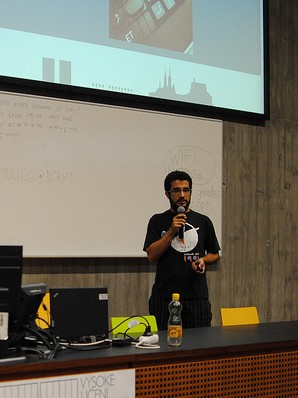
\includegraphics[width=0.275\textwidth]{img/guadec_2013_1.jpg}
    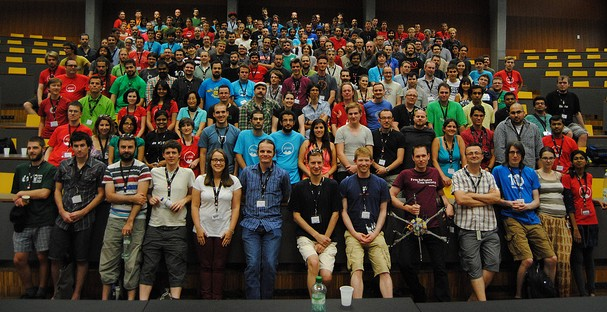
\includegraphics[width=0.715\textwidth]{img/guadec_2013_2.jpg}
    \caption{GUADEC 2013 (Brno)}
    \label{fig:guadec2012}
\end{figure}

Ademais de presentar o proxecto nesta xuntanza participei no evento como voluntario o que me permitiu coñecer a moita xente converténdose nunha experiencia moi enriquecedora tanto profesional como persoalmente.

\subsubsection{Reportes e Feedback}

A Fundación GNOME ponse en contacto comigo a través do email para pedirme que, xa que esta vai ser o aplicativo oficial de GNOME, ten que ter a palabra GNOME no seu nome.

Escribíronse dous reportes un\footnote{\href{http://aquelando.info/guadec-2013/}{GUADEC 2013}} falando da miña experiencia na GUADEC e outro\footnote{\href{http://aquelando.info/searching/}{Searching...}} falando dos avances no programa e pedindo ideas para o novo nome do aplicativo. Daniel Mustieles responde que ``GNOME Translator'' ou ``GNOME Translation Tool'' serían boas opcións.

\subsubsection{Tarefas e seguimento}

A descomposición en tarefas desta iteración é a seguinte:

\begin{enumerate}[label=\bfseries WBS 3.\arabic*]
  \item Deseño e implementación dos iteradores.
  \item Deseño e implementación do sistema de busca.
  \item Interface de usuario.
    \begin{enumerate}[label=\bfseries WBS 2.3.\arabic*]
      \item Resaltado do texto ao facer click nos consellos.
      \item Modificar editor de mensaxes
    \end {enumerate}
  \item Escribir reportes.
\end{enumerate}

Na Figura~\ref{fig:gantt:gsoc1-3} pódese ver o diagrama de Gantt correspondente as tarefas desta iteración.

\begin{figure}[h!]
\centerline{
\begin{ganttchart}[
    %hgrid,
    %inline,
    vgrid={dotted,dashed,dashed,dotted,dotted,dotted,dotted},
    x unit=5mm,
    y unit title=5mm,
    y unit chart=6mm,
    canvas/.style={draw=none},
    time slot format=isodate,
    title/.style={fill=gray, draw=none},
    title label font= \color{white}\scriptsize,
    title left shift=.1,
    title right shift=-.1,
    title top shift=.05,
    title height=.5,
    bar label font=\scriptsize,
    milestone label font=\scriptsize,
    group label font=\scriptsize\bfseries,
    %milestone inline label node/.append style={bottom=5mm},
    %group inline label node/.append style={right=0mm},
    %bar inline label node/.append style={right=0mm}
  ]{2013-07-18}{2013-8-06}
  \gantttitlecalendar{month=name,day} \\
  \ganttbar{Deseño e implementación dos iteradores}{2013-07-18}{2013-07-18} \ganttbar{}{2013-07-21}{2013-07-23} \\
  \ganttbar{Deseño e implementación do sistema de busca}{2013-07-24}{2013-07-25} \ganttbar{}{2013-07-28}{2013-07-29} \\
  \ganttgroup{Interface de usuario}{2013-07-30}{2013-08-4} \\
  \ganttbar{Resaltado do texto ao facer click nos consellos}{2013-07-30}{2013-07-31} \\
  \ganttbar{Modificar editor de mensaxes}{2013-08-1}{2013-08-1}  \ganttbar{}{2013-08-4}{2013-08-4} \\
  \ganttbar{Escribir reportes}{2013-8-5}{2013-8-5} \\
  \ganttlinkedmilestone{Fin terceira iteración}{2013-08-5}{2013-8-5}
\end{ganttchart}}
\caption{Diagrama de Gantt da terceira iteración do GSoC 2013.}
\label{fig:gantt:gsoc1-3}
\end{figure}

Esta iteración planificouse para un total de 65 horas. Nesta ocasión non houbo ningún problema e puideronse executar as tarefas no tempo previsto.

\subsection{Cuarta Iteración: Ficheiros po, Autools, Proxectos, barra de busca}
Esta iteración comeza o 6 de Agosto e remata o 30 do mesmo mes. O obxetivo desta iteración é engadir soporte para ficheiros po, proxectos, autotools e engadir unha barra de busca a interface.

\paragraph{Ficheiros PO}
O obxectivo consiste en implementar o soporte para ficheiros PO pois ata ese momento estábase empregando un mock. Crearanse bindings para a biblioteca gettext-po e implementarase unha subclase da clase abstracta File.

\paragraph{Proxectos}
Durante esta iteración tamén se implementarán os proxectos, definindo proxecto como un conxunto de ficheiros que están na mesma carpeta.

\paragraph{Autotools}
Implementarase tamén o soporte para autotools do proxecto pois ata o momento víñase a empregar un simple ficheiro Makefile.

\paragraph{Interface de usuario}
Crearanse accións para facer e desfacer cambios, navegar a través do documento entre outras cousas. Estas accións poderán ser activadas a través de botóns na interface de usuario ou mediante atallos de teclado que se crearán posteriormente. Ademais engadirase o soporte para abrir ficheiros dende a propia interface e a posibilidade de ver os ficheiros recentes.

\subsubsection{Reportes e feedback}

Falando co anterior \emph{maintainer} de GTranslator a través de IRC, este aporta bastantes consellos sobre o programa como o uso de Autotools ou varios detalles da interface de usuario.

Realizáronse un total de dous reportes\footnote{\href{http://aquelando.info/gsoc-application-status-report/}{GSoC application status report}}\footnote{\href{http://aquelando.info/po-files-projects-navigation-and-other-stuff-i-have-been-doing/}{Po files, projects, navigation and other stuff I have been doing}} pero ninguén escribiu ningún comentario no blogue.

\subsubsection{Tarefas e Seguimento}

As tarefas que se realizaron durante esta iteración foron as seguintes:

\begin{enumerate}[label=\bfseries WBS 4.\arabic*]
  \item Implementación dos ficheiros po.
  \item Implementación de proxectos
  \item Implementación de accións
    \begin{enumerate}[label=\bfseries WBS 4.3.\arabic*]
      \item Accións desfacer-refacer
      \item Accións de navegar polo documento.
    \end{enumerate}
  \item Engadir barra de busca.
  \item Eliminar barra de estado.
  \item Substituir Makefile por Autools.
  \item Internacionalización do programa.
  \item Escribir reportes.
\end {enumerate}

Na Figura~\ref{fig:gantt:gsoc1-4} pódese ver o diagrama de Gantt correspondente a esta iteración.

\begin{figure}[h!]
\centerline{
\begin{ganttchart}[
    %hgrid,
    %inline,
    vgrid={dotted,dotted,dotted,dotted,dotted,dashed,dashed},
    x unit=4.5mm,
    y unit title=5mm,
    y unit chart=6mm,
    canvas/.style={draw=none},
    time slot format=isodate,
    title/.style={fill=gray, draw=none},
    title label font= \color{white}\scriptsize,
    title left shift=.1,
    title right shift=-.1,
    title top shift=.05,
    title height=.5,
    bar label font=\scriptsize,
    milestone label font=\scriptsize,
    group label font=\scriptsize\bfseries,
    %milestone inline label node/.append style={bottom=5mm},
    %group inline label node/.append style={right=0mm},
    %bar inline label node/.append style={right=0mm}
  ]{2013-08-5}{2013-8-30}
  \gantttitlecalendar{month=name,day} \\
  \ganttbar{Implementación dos ficheiros PO}{2013-08-5}{2013-08-9}  \ganttbar{}{2013-08-12}{2013-08-13} \\
  \ganttbar{Implementación de proxectos}{2013-08-14}{2013-08-14} \\
  \ganttgroup{Implementación de accións}{2013-08-15}{2013-08-16} \\
  \ganttbar{Accións desfacer-refacer}{2013-08-15}{2013-08-15} \\
  \ganttbar{Accións de navegar}{2013-08-16}{2013-08-16} \\
  \ganttgroup{Interface de Usuario}{2013-08-19}{2013-08-21} \\
  \ganttbar{Engadir barra de busca}{2013-08-19}{2013-08-20} \\
  \ganttbar{Eliminar barra de estado}{2013-08-21}{2013-08-21} \\
  \ganttbar{Creacion de scripts de Autools}{2013-08-22}{2013-08-23} \ganttbar{}{2013-08-26}{2013-08-28} \\
  \ganttbar{Internacionalización}{2013-08-29}{2013-08-29} \\
  \ganttbar{Escribir reportes}{2013-08-30}{2013-08-30} \\
  \ganttmilestone{Fin cuarta iteración}{2013-08-30}
\end{ganttchart}}
\caption{Diagrama de Gantt da cuarta iteración do GSoC 2013.}
\label{fig:gantt:gsoc1-4}
\end{figure}

Planificáronse un total 100 horas para esta iteración. Tardamos 5 horas máis das previstas en implementar o soporte para Autotools e outras 5 horas adicionais por problemas encontrados na implementación dos bindings da biblioteca de GetText. De igual forma que nos casos anteriores estes problemas resolveronse ampliando a xornada laboral.

\subsection{Quinta Iteración: Preferencias, limpar código e documentación}
Esta iteración comeza o 1 de septembro e remata o 23 do mesmo mes. Durante ela seguirase traballando na interface, limparase o código e crearase algo de documentación de cara a entrega final do Google Summer of Code.

\paragraph{Preferencias}
Empezarase a implementar as preferencias no programa pois ata o momento moitas das opcións estaban \emph{hardcoded}, e dicir escritas directamente no código. Para facer isto farase uso do compoñente de GLib GSettings que permite o almacenamento sinxelo de configuración das aplicacións. Ademais implementarase un dialogo semellante ao empregado en GTranslator para poder modificar estas preferencias.

\paragraph{Mellorar a calidade do código e documentación}
Revisión completa do código para manter un mesmo estilo ao largo de todo o código. Ademais actualizáronse os diagramas UML creados na primeira iteración.

\subsubsection{Reportes e Feedback}
Escribiuse un\footnote{\href{http://aquelando.info/gsoc-final-report/}{GSoC Final Report}} reporte onde se conta o estado da aplicación demostrándoo con un vídeo. O tratarse do último post desa edición do GSoC agradezo a oportunidade que me deu Google para poder estar ese verán traballando en software libre e describo a miña experiencia.

\subsubsection{Tarefas e seguimento}

As tarefas realizadas durante esta iteración foron as seguintes:

\begin{enumerate}[label=\bfseries WBS 5.\arabic*]
  \item Deseño e implementación das preferencias.
  \item Corrixir Clase ficheiro.
  \item Corrixir errores de estilos no código.
  \item Actualizar diagramas UML.
  \item Escribir reportes.
\end {enumerate}

Hai que ter en conta que nesta iteración a cantidade de tempo traballada por día é inferior nalgúns momentos pois en que compatibilizarse co horario lectivo do curso 2013/2014. Na Figura~\ref{fig:gantt:gsoc1-5} pódese ver o diagrama de Gantt que corresponde a esta iteración.

\begin{figure}[h!]
\centerline{
\begin{ganttchart}[
    %hgrid,
    %inline,
    vgrid={dashed,dotted,dotted,dotted,dotted,dotted,dashed},
    x unit=4.5mm,
    y unit title=5mm,
    y unit chart=6mm,
    canvas/.style={draw=none},
    time slot format=isodate,
    title/.style={fill=gray, draw=none},
    title label font= \color{white}\scriptsize,
    title left shift=.1,
    title right shift=-.1,
    title top shift=.05,
    title height=.5,
    bar label font=\scriptsize,
    milestone label font=\scriptsize,
    group label font=\scriptsize\bfseries,
    %milestone inline label node/.append style={bottom=5mm},
    %group inline label node/.append style={right=0mm},
    %bar inline label node/.append style={right=0mm}
  ]{2013-09-1}{2013-9-24}
  \gantttitlecalendar{month=name,day} \\
  \ganttbar{Deseño e implementación das preferencias}{2013-09-2}{2013-09-6} \ganttbar{}{2013-09-9}{2013-09-10} \\
  \ganttbar{Corrixir Clase ficheiro}{2013-09-11}{2013-09-13}  \ganttbar{}{2013-09-16}{2013-09-17} \\
  \ganttbar{Corrixir errores de estilos no código}{2013-09-18}{2013-09-18} \\ 
  \ganttbar{Actualizar diagramas UML}{2013-09-19}{2013-09-20} \\
  \ganttbar{Escribir reportes}{2013-09-23}{2013-09-23} \\
  \ganttmilestone{Fin quinta iteración}{2013-09-23}
\end{ganttchart}}
\caption{Diagrama de Gantt da quinta iteración do GSoC 2013.}
\label{fig:gantt:gsoc1-5}
\end{figure}

Planificaronse un total de 60 horas para resolver as tarefas e non houbo ningún problema en completalas con éxito.

\subsection{Estado ao fin do GSoC 2013}
O finalizar esta iteración o mentor do GSoC avalía correctamente o proxecto presentado polo que o programa é completado con éxito. O programa entregado ten entre outras moitas as seguintes características:

\begin{itemize}
  \item Posibilidade de abrir ficheiros po.
  \item Navegación a través do documento.
  \item Posibilidade de buscar.
  \item Editor con resaltado de sintaxe e de espazos en branco.
  \item Preferencias.
\end{itemize}

Pero tamén presenta algúns fallos:

\begin{itemize}
  \item Lentitude ao cargar ficheiros moi grandes.
  \item Fallo ao gardar un ficheiro.
  \item O aspecto da interface non é satisfactorio.
  \item Problemas ao buscar.
\end{itemize}

Estas limitacións serán eliminadas durante os seguintes períodos.


\section{Primeiro cuatrimestre curso 2013/2014}

Durante este período a implementación do programa faise en paralelo coa vida universitaria. Planifícanse dúas iteracións, a primeira durante o que falta do mes de setembro e o mes de outubro e a segunda durante o final do mes de nobembro. Nestes dous periodos de tempo a carga de traballo das tarefas das materias do curso 2013/2014 é menor e permitenos continuar traballando coa aplicación.

\subsection{Primeira iteración: cambios na interface}
A primeira iteración comprende os últimos días de setembro e o mes de outubro. Durante este tempo farase un redeseño da interface gráfica e implementanse as pistas e os comprobadores:

\paragraph{Interface Gráfica} Pretendese conseguir un mellor resultado do actual. Empregaremos os deseños iniciais que teñen un parecido máis importante a aplicación Virtaal. Reutilizarase os widgets creados combinándoos para conseguir o efecto desexado.


\paragraph{Pistas e Comprobadores} As pistas (\emph{hints}) son posibles traducións para unha cadea determinada. Nesta iteración crearase tanto o panel da interface que permite ver estas pistas como a clase que lle prove as pistas a dita interface. Os comprobadores (\emph{checkers}), por outro lado, apórtanlle pistas de cada tradución feita.

\subsubsection{Presentación GUADEC Hispana 2013 (Madrid)}

A GUADEC Hispana é unha reunión de usuarios e desenvolvedores de GNOME de fala castelá e que serve tamén para a reunión anual (como obriga a lei) da organización GNOME Hispano. Ademais nesta reunión fanse charlas sobre GNOME e outros temas relacionados.

\begin{figure}[h!]
    \centering
    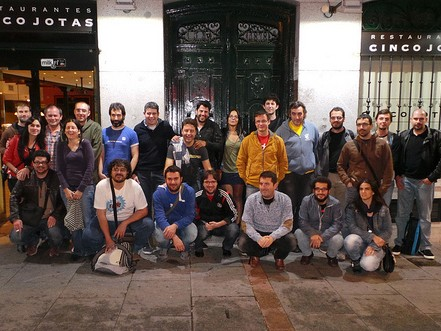
\includegraphics[width=0.495\textwidth]{img/guadec_es_2013_1.jpg}
    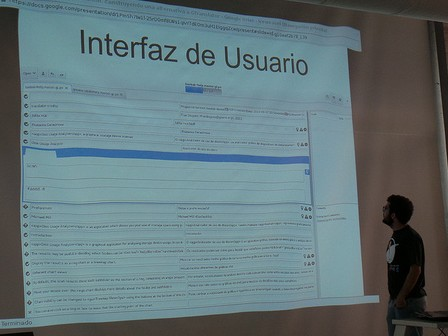
\includegraphics[width=0.495\textwidth]{img/guadec_es_2013_2.jpg}
    \caption{GUADEC Hispana 2013 (Madrid)}
    \label{fig:guadec2012}
\end{figure}

Entre esas charlas tiven a oportunidade de presentar o proxecto polo que os asistentes amosaron o seu interese por que se seguira desenrolando.

\subsubsection{Reportes e feedback}
Escribiuse un reporte\footnote{\href{http://aquelando.info/changing-the-tool-ui/}{Changing the tool UI}} mais ninguén escribiu ningún comentario. Non obstante durante a GUADEC-es houbo xente que se interesou polo programa.

\subsubsection{Tarefas e seguimento}

A descomposición en tarefas para esta iteración é a seguinte:

\begin{enumerate}[label=\bfseries WBS 1.\arabic*]
  \item Implementar Pistas e Provedor de Pistas.
  \item Implementar Comprobador.
  \item Interface de Usuario.
    \begin{enumerate}[label=\bfseries WBS 1.3.\arabic*]
      \item Eliminar biblioteca GDL.
      \item Engadir widget de Pistas.
      \item Misturar lista de mensaxes con editor de mensaxes.
    \end{enumerate}
\end{enumerate}

Hai que ter en conta que ao ter que compatibilizar a realización destas tarefas co horario acadameico o número de horas traballadas cada día é menor que no periodo anterior e non é regular. Na Figura~\ref{fig:gantt:mid1-1} pódese ver o diagrama de Gantt que corresponde a esta iteración.

\begin{figure}[h!]
\centerline{
\begin{ganttchart}[
    vgrid={dotted,dotted,dashed,dashed,dotted,dotted,dotted},
    x unit=4.5mm,
    y unit title=5mm,
    y unit chart=6mm,
    canvas/.style={draw=none},
    time slot format=isodate,
    title/.style={fill=gray, draw=none},
    title label font= \color{white}\scriptsize,
    title left shift=.1,
    title right shift=-.1,
    title top shift=.05,
    title height=.5,
    bar label font=\scriptsize,
    milestone label font=\scriptsize,
    group label font=\scriptsize\bfseries
  ]{2013-09-26}{2013-10-20}
  \gantttitlecalendar{month=name,day} \\
  \ganttbar{Implementar Pistas}{2013-09-26}{2013-09-27} \\
  \ganttbar{Implementar Provedor de Pistas}{2013-09-30}{2013-10-1} \\
  \ganttbar{Implementar Comprobador}{2013-10-2}{2013-10-3} \\
  \ganttgroup{Interface de Usuario}{2013-10-4}{2013-10-17} \\
  \ganttbar{Eliminar biblioteca GDL}{2013-10-4}{2013-10-4}  \ganttbar{}{2013-10-7}{2013-10-8} \\
  \ganttbar{Engadir widget de Pistas}{2013-10-9}{2013-10-11} \\
  \ganttbar{Reimplementar lista de mensaxes}{2013-10-14}{2013-10-17} \\
  \ganttbar{Escribir reportes}{2013-10-18}{2013-10-18} \\
  \ganttmilestone{Fin iteración}{2013-10-18}
\end{ganttchart}}
\caption{Diagrama de Gantt da primeira iteración do primeiro cuatrimestre do curso 2013/2014.}
\label{fig:gantt:mid1-1}
\end{figure}

Para a realización destas tarefas planificáronse 50 horas que se completaron con éxito.

\subsection{Segunda iteración: Refactorizar navegadores e melloras na interface}
Esta iteración sucede no final do mes de novembro. Durante este tempo cambiaraselle o nome ao aplicativo, refactorízase a API para navegar a través do documento e realízaranse pequenos cambios na interface de usuario.

\paragraph{Refactorización dos navegadores} Crearase unha API a nivel de aplicación para movernos a través do documento. O obxectivo é implementar operacións para seleccionar e tamén deseleccionar cadeas e fragmentos destas cadeas a través de todo o documento.

\paragraph{Cambio de nome} Reutilizarase un cambio de nome do aplicativo cambiando o anterior ValaCAT por GNOMECAT. Este cambio é producido polo requirimento por parte da fundación GNOME de que o programa tiña que ter a marca GNOME no seu nome.

\paragraph{Interface de usuario} Farase un redeseño a opción de buscar avanzado para eliminar o dialogo existente e engadir as opción existentes a propia barra de busca.

\subsubsection{Reportes e Feedback}
Escríbese un\footnote{\href{http://aquelando.info/welcome-gnomecat/}{Welcome GnomeCAT}} contando os últimos avances do aplicativo e o cambio de nome. Recibimos un comentario dicindo que GNOME escribese con letras maiúsculas polo que temos que corrixir o programa. Outra xente interesase polo significado de CAT.

\subsubsection{Tarefas e seguimento}

As tarefas realizadas durante esta iteración foron as seguintes:

\begin{enumerate}[label=\bfseries WBS 2.\arabic*]
  \item Cambiar nome do aplicativo.
  \item Refactorizar navegadores.
  \item Interface de usuario.
    \begin{enumerate}[label=\bfseries WBS 2.3.\arabic*]
      \item Redeseño da opción buscar avanzado.
    \end{enumerate}
\end{enumerate}

De igual forma que no caso anterior o feito de estar dentro do periodo lectivo, causa que o número de horas traballadas sexa menor do normal. Na Figura~\ref{fig:gantt:mid1-2} pódese ver o diagrama de Gantt que corresponde a esta iteración.

\begin{figure}[h!]
\centerline{
\begin{ganttchart}[
    vgrid={dotted,dotted,dotted,dotted,dotted,dashed,dashed},
    x unit=4.5mm,
    y unit title=5mm,
    y unit chart=6mm,
    canvas/.style={draw=none},
    time slot format=isodate,
    title/.style={fill=gray, draw=none},
    title label font= \color{white}\scriptsize,
    title left shift=.1,
    title right shift=-.1,
    title top shift=.05,
    title height=.5,
    bar label font=\scriptsize,
    milestone label font=\scriptsize,
    group label font=\scriptsize\bfseries
  ]{2013-11-18}{2013-11-30}
  \gantttitlecalendar{month=name,day} \\
  \ganttbar{Cambiar nome do aplicativo}{2013-11-18}{2013-11-19} \\
  \ganttbar{Refactorizar navegadores}{2013-11-20}{2013-11-22} \\
  \ganttgroup{Interface de usuario}{2013-11-25}{2013-11-28} \\
  \ganttbar{Redeseño da opción buscar avanzado}{2013-11-25}{2013-11-28} \\
  \ganttbar{Escribir reportes}{2013-11-29}{2013-11-29} \\
  \ganttmilestone{Fin segunda iteración}{2013-11-29}
\end{ganttchart}}
\caption{Diagrama de Gantt da segunda iteración do primeiro cuatrimestre do curso 2013/2014.}
\label{fig:gantt:mid1-2}
\end{figure}

Para a realización das tarefas descritas planificanse 35 horas que son suficientes para completalas nos días estipulados.

\subsection{Presentación para o GSoC 2014}
Debido a evidente falta de tempo para completar o programa decídese presentar o programa de novo o proxecto Google Summer of Code. Falase coa coordinadora dos programas de iniciación en GNOME para saber se isto é posible e respóndenos afirmativamente. Como mentor falamos co \emph{maintainer} de GTranslator que nos di que non ten ningún problema en facer de mentor. Presentamos o proxecto e este sae aceptado.

\section{Google Summer of Code 2014}
O Google Summer of Code durante o 2014 dura dende o 19 de maio ata o 11 de agosto un total de 15 semanas. Na planificación realizada cóntanse 13 semanas pois nunha das semanas o curso lectivo 2013/2014 aínda non acabou e na outra realizase o viaxe a GUADEC en Strasbourg. Da mesma forma que no caso anterior planéanse traballar 5 horas diarias o que da un total de 325 horas.

A maior experiencia no programa que estamos a facer permítenos facer unha planificación máis exacta. Faranse un total de cinco iteración de unha duración aproximada de dúas semanas.

\subsection{Primeira iteración: Redeseño UI}

Esta iteración dura dende o 23 de maio ata o 15 xuño. Durante ela fundamentalmente traballaremos nun redeseño da interface.

\paragraph{Interface Gráfica} O obxectivo desta iteración é un novo redeseño da interface. Contactarase cos deseñadores de GNOME a través de IRC para obter algún feedback pola súa parte. Unha vez conseguido, implementarase a nova interface.

\paragraph{Bindings Gettext-PO: Orixes das mensaxes}
A biblioteca gettext-po ten soporte para conseguir os orixes das mensaxes. Nesta iteración tamén se mellorarán os seus bindings para recoller esta característica e tamén a implementaremos na clase PoFile engadindo a propiedade origins que permite obter en que ficheiros e liñas aparece dita cadea.

\subsubsection{Reportes e Feedback}
Escribíronse dous\footnote{\href{http://aquelando.info/gnomecat-progress-report/}{GNOMECAT. Progress report}}\footnote{\href{http://aquelando.info/implementing-the-editing-panel/}{Implementing the Editing Panel}} reportes. En esta iteración hai bastante resposta por parte do usuario. Por unha parte reportase un erro na compilación do programa respondémoslle ao usuario dándolle un \emph{workaround} mentras buscamos o motivo real do problema.

Ademais, o deseñador que fixo os mockups empregados agradece que os esteamos usando e sinala que sería boa idea substituir o menú de selección de idioma actual por algo máis vistoso. Tamén sinala que quedaría ben combinar os botóns de gardar e de volver atrás de forma que un usuario so poida volver a lista de ficheiros abertos cando o ficheiro que está traballando. Anotamos estas dúas ideas en GitHub para implementalas máis tarde.

\subsubsection{Tarefas e seguimento}

As tarefas realizadas durante esta iteración foron:

\begin{enumerate}[label=\bfseries WBS 1.\arabic*]
  \item Creación do ficheiro .desktop.
  \item Mellora de Autotools: xeneración automática das cadeas a traducir.
  \item Interface de Usuario.
    \begin{enumerate}[label=\bfseries WBS 1.3.\arabic*]
      \item Nova estrutura xeral.
      \item Creación da barra de ferramentas.
      \item Panel de edición.
      \item Panel de preferencias.
      \item Panel de perfil.
      \item Panel de benvida.
      \item Menú de aplicativo.
    \end{enumerate}
  \item Bindings Gettext-PO: implementación das orixes dos mensaxes.
  \item Refactorización das buscas.
  \item Refactorización as formas plurais.
\end{enumerate}

Na Figura~\ref{fig:gantt:gsoc2014-1} pódese ver o diagrama de Gantt que corresponde a esta iteración.

\begin{figure}[h!]
\centerline{
\begin{ganttchart}[
    vgrid={dotted,dotted,dashed,dashed,dotted,dotted,dotted},
    x unit=4.5mm,
    y unit title=5mm,
    y unit chart=6mm,
    canvas/.style={draw=none},
    time slot format=isodate,
    title/.style={fill=gray, draw=none},
    title label font= \color{white}\scriptsize,
    title left shift=.1,
    title right shift=-.1,
    title top shift=.05,
    title height=.5,
    bar label font=\scriptsize,
    milestone label font=\scriptsize,
    group label font=\scriptsize\bfseries
  ]{2014-05-22}{2014-6-15}
  \gantttitlecalendar{month=name,day} \\
  \ganttbar{Creación do ficheiro .desktop}{2014-05-23}{2014-05-23} \\
  \ganttgroup{Autotools}{2014-05-26}{2014-05-26} \\
  \ganttbar{Xeneración automática das cadeas a traducir}{2014-05-26}{2014-05-26} \\
  \ganttgroup{Interface de Usuario}{2014-05-27}{2014-06-9} \\
  \ganttbar{Nova estrutura xeral}{2014-05-27}{2014-05-28} \\
  \ganttbar{Creación da barra de ferramentas}{2014-05-29}{2014-05-30} \\
  \ganttbar{Panel de edición}{2014-06-2}{2014-06-3} \\
  \ganttbar{Panel de preferencias}{2014-06-4}{2014-06-4} \\
  \ganttbar{Panel de perfil}{2014-06-5}{2014-06-5} \\
  \ganttbar{Panel de benvida}{2014-06-6}{2014-06-6} \\
  \ganttbar{Menú de aplicativo}{2014-06-9}{2014-06-9} \\
  \ganttgroup{Bindings Gettext-PO}{2014-06-10}{2014-06-10} \\
  \ganttbar{Implementación das orixes dos mensaxes}{2014-06-10}{2014-6-10} \\
  \ganttbar{Refactorización das buscas}{2014-06-11}{2014-06-11} \\
  \ganttbar{Refactorización as formas plurais}{2014-6-12}{2014-6-12} \\
  \ganttbar{Escribir reportes}{2014-06-13}{2014-06-13} \\
  \ganttmilestone{Fin da primeira iteración}{2014-6-13}
\end{ganttchart}}
\caption{Diagrama de Gantt da primeira iteración do GSoC 2014.}
\label{fig:gantt:gsoc2014-1}
\end{figure}

Para facer as tarefas anteriores planifícanse un total de 80 horas. Non son necesarias horas adicionais nesta ocasión.

\subsection{Segunda Iteración: Bindings Gettext-PO e interface}
Esta iteración dura dende o 15 de xuño ata o 6 de xuño. Continuamos mellorando a interface de usuario, implementamos atallos de teclado e engadimos funcionalidade aos bindings de Gettext-PO.

\paragraph{Interface de usuario} Traballarase en implementar atallos de teclado e mellorar o panel de editar perfiles de usuarios dividindo o panel en dous subpaneis. Por último engadirase na interface a opción de obter os orixes de cada mensaxe.

\paragraph{Bindings Gettext-PO} Implementación da opción de modificar as cabeceiras dos ficheiros PO aparte de solucionar algúns erros detectados.

\subsubsection{Reportes e Feedback}

Escríbese un\footnote{\href{http://aquelando.info/keep-working-on-gnomecat/}{Keep working on GNOMECAT}} reporte. So recibimos un comentario sinalando que sería interesante que durante a GUADEC falase con un dos desenvolvedores de GNOME.

\subsubsection{Tarefas e seguimento}

As tarefas realizadas durante esta iteración foron:

\begin{enumerate}[label=\bfseries WBS 2.\arabic*]
  \item Interface de Usuario.
    \begin{enumerate}[label=\bfseries WBS 2.1.\arabic*]
      \item Atallos de teclado.
      \item Widget de Pistas.
      \item Orixes das cadeas.
      \item Mellorar Panel de Perfil.
      \item Mellorar Panel Abrir Ficheiro.
    \end{enumerate}
  \item Arreglar Buscas.
  \item Bindings Gettext-PO.
    \begin{enumerate}[label=\bfseries WBS 2.3.\arabic*]
      \item Xestión de cabeceiras.
      \item Gardado de ficheiros.
    \end{enumerate}
  \item Escribir reportes.
\end{enumerate}

Na Figura~\ref{fig:gantt:gsoc2014-2} pódese ver o diagrama de Gantt que corresponde a esta iteración.

\begin{figure}[h!]
\centerline{
\begin{ganttchart}[
    vgrid={dashed,dotted,dotted,dotted,dotted,dotted,dashed},
    x unit=4.5mm,
    y unit title=5mm,
    y unit chart=6mm,
    canvas/.style={draw=none},
    time slot format=isodate,
    title/.style={fill=gray, draw=none},
    title label font= \color{white}\scriptsize,
    title left shift=.1,
    title right shift=-.1,
    title top shift=.05,
    title height=.5,
    bar label font=\scriptsize,
    milestone label font=\scriptsize,
    group label font=\scriptsize\bfseries
  ]{2014-06-15}{2014-7-6}
  \gantttitlecalendar{month=name,day} \\
  \ganttgroup{Interface de Usuario}{2014-06-16}{2014-06-26} \\
  \ganttbar{Atallos de teclado}{2014-06-16}{2014-06-17} \\
  \ganttbar{Widget de Pistas}{2014-06-18}{2014-06-19} \\
  \ganttbar{Orixes das cadeas}{2014-06-20}{2014-06-20} \\
  \ganttbar{Mellorar Panel Perfil}{2014-6-23}{2014-6-24} \\
  \ganttbar{Mellorar Panel Abrir Ficheiro}{2014-6-25}{2014-6-26} \\
  \ganttbar{Arreglar buscas}{2014-06-27}{2014-06-27} \\
  \ganttgroup{Bindings Gettext-PO}{2014-06-30}{2014-07-3} \\
  \ganttbar{Xestión de cabeceiras}{2014-06-30}{2014-07-1} \\
  \ganttbar{Gardado de ficheiros}{2014-07-2}{2014-07-3} \\
  \ganttbar{Escribir reportes}{2014-7-4}{2014-7-4} \\
  \ganttmilestone{Fin Segunda iteración}{2014-7-4}
\end{ganttchart}}
\caption{Diagrama de Gantt da segunda iteración do GSoC 2014.}
\label{fig:gantt:gsoc2014-2}
\end{figure}

Planificamos un total de 75 horas para esta iteración. Necesitamos 3 horas adicionais para resolver algúns problemas encontrados coa implementación dos bindings para a biblioteca Gettext-PO.

\subsection{Terceira Iteración: Perfiles de usuario e interface}
Esta iteración dura dende o 7 de Xullo ao 16 do mesmo mes. Melloramos algo a interface de usuario e implementamos algún detalle que faltaba no sistema de perfiles.

\paragraph{Interface de usuario: Barra de notificación} Implementarase un sistema de notificacións para alertar ao usuario de certos eventos no programa como por exemplo cando os parámetros de busca non xeran ningún resultado. Para iso empregaremos o widget de GTK GtkInfoBar que amosaremos durante 3 segundos.

\paragraph{Perfiles de usuario} Implementarase a funcionalidade de activar perfiles e engadirase un botón a interface para permitir borrar e activar perfiles.

\subsubsection{Reportes e Feedback}

Escribese un\footnote{\href{http://aquelando.info/details-and-more-details/}{Details and more details}} reporte pero non recibimos feedback por parte dos tradutores nesta iteración.

\subsubsection{Tarefas e seguimento}

As tarefas realizadas durante esta iteración foron:

\begin{enumerate}[label=\bfseries WBS 3.\arabic*]
  \item Interface de usuario: barra de notificación.
  \item Perfiles de usuario.
    \begin{enumerate}[label=\bfseries WBS 3.2\arabic*]
      \item Función borrar perfil.
      \item Función activar perfil.
    \end{enumerate}
  \item Modificar ficheiro das formas plurais.
\end{enumerate}

Na Figura~\ref{fig:gantt:gsoc2014-3} pódese ver o diagrama de Gantt que corresponde a esta iteración.

\begin{figure}[h!]
\begin{ganttchart}[
    vgrid={dashed,dashed,dotted,dotted,dotted,dotted,dotted},
    x unit=4.5mm,
    y unit title=5mm,
    y unit chart=6mm,
    canvas/.style={draw=none},
    time slot format=isodate,
    title/.style={fill=gray, draw=none},
    title label font= \color{white}\scriptsize,
    title left shift=.1,
    title right shift=-.1,
    title top shift=.05,
    title height=.5,
    bar label font=\scriptsize,
    milestone label font=\scriptsize,
    group label font=\scriptsize\bfseries
  ]{2014-07-5}{2014-7-17}
  \gantttitlecalendar{month=name,day} \\
  \ganttgroup{Interface de usuario}{2014-07-7}{2014-07-7} \\
  \ganttbar{Barra de notificación}{2014-07-7}{2014-07-7} \\
  \ganttgroup{Perfiles de usuario}{2014-07-8}{2014-07-10} \\
  \ganttbar{Función borrar perfil}{2014-07-8}{2014-07-8} \\
  \ganttbar{Función activar perfil}{2014-07-9}{2014-07-10} \\
  \ganttgroup{Refactorizar API Formas Plurais}{2014-07-11}{2014-7-11} \\
  \ganttbar{Modificar ficheiro das formas plurais}{2014-7-11}{2014-7-11} \\
  \ganttbar{Mellorar Busca}{2014-07-14}{2014-07-15} \\
  \ganttbar{Escribir reportes}{2014-07-16}{2014-07-16} \\
  \ganttmilestone{Fin terceira iteración}{2014-7-16}
\end{ganttchart}
\caption{Diagrama de Gantt da terceira iteración do GSoC 2014.}
\label{fig:gantt:gsoc2014-3}
\end{figure}

Para completar as tarefas anteriores planificamos 40 horas que foron suficientes para conseguir rematar as tarefas con éxito.

\subsection{Cuarta Iteración: Plugins e GUADEC}
Esta iteración dura dende o 16 de Xullo ata o 5 de Agosto tendo a GUADEC polo medio. Conseguimos implementar o motor de plugins e creamos algúns plugins de exemplo.

\paragraph{Plugins} Engadiremos o soporte de plugins o programa. Por unha parte incorporaremos un motor de plugins e refactorizaremos o código para que certas partes do mesmo deixen de depender da interface de usuario. Ademais modificaremos a configuración de Autotools para que compile os plugins.

\subsubsection{Presentación GUADEC 2014 (Strasbourg)}
Da mesma forma que na edición anterior acudimos a GUADEC, a reunión de programadores e usuarios de GNOME en Europa. Desta vez celébrase en Strasbourg.

\begin{figure}[h!]
    \centering
    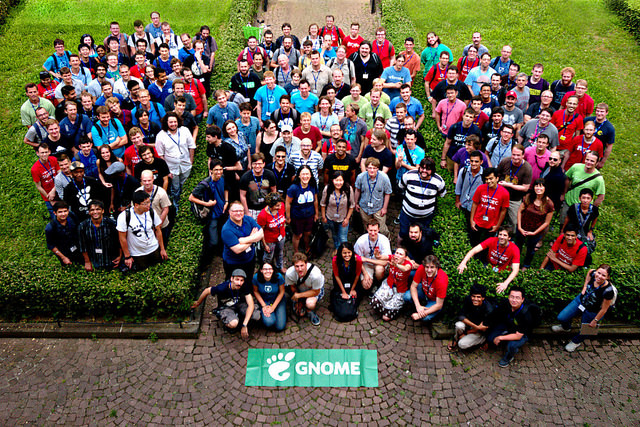
\includegraphics[width=0.999\textwidth]{img/guadec_2014.jpg}
    \caption{GUADEC 2014 (Strasbourg)}
    \label{fig:guadec2012}
\end{figure}

Tamén temos a oportunidade de presentar o proxecto ante a comunidade GNOME nunha charla lóstrego de 3 minutos onde explicaremos os novos cambios na interface, a implementación e plugins e as novas características implementadas.

\subsubsection{Reportes e Feedback}

Escribese un\footnote{\href{http://aquelando.info/api-guadec-and-big-files/}{API, GUADEC and big files}} reporte. Ninguén fai un comentario no blogue sobre o programa pero durante a GUADEC fálase con algún desenvolvedor que nos da consellos sobre algún dos problemas que temos. Marina Zhurakhinskaya recoméndanos falar con Allan Day que é o deseñador líder de GNOME para que nos diga se hai algo que debemos mellorar no deseño do aplicativo.

\subsubsection{Tarefas e seguimento}

As tarefas realizadas duarnte esta iteración foron:

\begin{enumerate}[label=\bfseries WBS 4.\arabic*]
  \item Melloras en Autools
  \item Interface de usuario: \emph{scrolling} nas buscas.
  \item Implementación de plugins.
  \item Refactorizar clase File: evitar dependencias coa interface.
\end{enumerate}

Na Figura~\ref{fig:gantt:gsoc2014-4} pódese ver o diagrama de Gantt que corresponde a esta iteración.

\begin{figure}[h!]
\centerline{
\begin{ganttchart}[
    vgrid={dotted,dotted,dotted,dashed,dashed,dotted,dotted},
    x unit=4.5mm,
    y unit title=5mm,
    y unit chart=6mm,
    canvas/.style={draw=none},
    time slot format=isodate,
    title/.style={fill=gray, draw=none},
    title label font= \color{white}\scriptsize,
    title left shift=.1,
    title right shift=-.1,
    title top shift=.05,
    title height=.5,
    bar label font=\scriptsize,
    milestone label font=\scriptsize,
    group label font=\scriptsize\bfseries
  ]{2013-7-16}{2013-8-6}
  \gantttitlecalendar{month=name,day} \\
  \ganttgroup{Implementación de plugins}{2013-07-16}{2013-07-25} \\
  \ganttbar{Implementación de motor de plugins}{2013-07-16}{2013-07-17} \\
  \ganttgroup{Biblioteca GNOMECAT}{2013-07-18}{2013-07-22} \\
  \ganttbar{Refactorizar clase File}{2013-07-18}{2013-07-18}  \ganttbar{}{2013-07-21}{2013-07-21} \\
  \ganttbar{Refactorizar clase Language}{2013-07-22}{2013-07-22} \\
  \ganttbar{Modificar Autotools para compilar plugins}{2013-07-23}{2013-07-23} \\
  \ganttbar{Plugin de exemplo de comprobador}{2013-07-24}{2013-07-24} \\
  \ganttbar{Plugin de exemplo de proveedor de suxerencias}{2013-07-25}{2013-07-25} \\
  \ganttbar{Refactorizar Navegadores}{2013-07-28}{2013-07-29} \\
  \ganttbar{Interface de usuario: scrolling nas buscas}{2013-07-30}{2013-07-31} \\
  \ganttbar{Mellorar o rendemento con ficheiros grandes}{2013-08-1}{2013-08-1}  \ganttbar{}{2013-08-4}{2013-08-4} \\
  \ganttbar{Escribir reportes}{2013-08-5}{2013-08-5} \\
  \ganttmilestone{Fin cuarta iteración}{2013-8-5}
\end{ganttchart}}
\caption{Diagrama de Gantt da cuarta iteración do GSoC 2014.}
\label{fig:gantt:gsoc2014-4}
\end{figure}

Planificamos 75 horas para as tarefas desta iteración. Precisamos 5 horas adicionais para modificar os scripts de Autotools que permiten a compilación dos plugins. Para non incrementar o número de días desta iteración aumentamos o número de horas que traballamos determinados días.


\subsection{Quinta Iteración: Detalles finais e escribir documentación}
Esta iteración dura dende o 5 de Agosto ata o 15 do mesmo mes. Nela puliremos algún detalle da interface e melloraremos a calidade do código e a documentación.

\paragraph{Documentación e limpar código} O obxectivo é facer unha revisión do código para que este manteña un mesmo estilo. Ademais actualizarase a documentación existente e crearase algunha nova.

\paragraph{Interface: Lista de mensaxes} Intentarase mellorar o rendemento da lista de mensaxes que detectamos que non funciona correctamente con ficheiros grandes. Este é un problema que temos dende a primeira edición do GSoC. Ademais engadiremos a función de filtrar e ordenar mensaxes.

\subsubsection{Reportes e Feedback}
Nesta ocasión non se escriben reportes mais si que recibimos feedback de algún tradutor a través do correo electrónico. As cousas que estes tradutores consideran que se deben mellorar son as seguintes:

\begin{itemize}
   \item Mellora dos atallos de teclado.
\end{itemize}

Ademais falamos con Allan Day que nos di que cando poida fará unha revisión da interface de usuario do programa.

\subsubsection{Tarefas e seguimento}

As tarefas realizadas durante esta iteración foron:

\begin{enumerate}[label=\bfseries WBS 5.\arabic*]
  \item Documentación.
  \item Limpar código.
  \item Interface de usuario: Refactorizar lista de mensaxes.
    \begin{enumerate}[label=\bfseries WBS 5.3.\arabic*]
      \item Implementar novo widget de lista de mensaxes.
      \item Implementar filtros para lista de mensaxes.
      \item Implementar a función de ordenar para mensaxes.
    \end{enumerate}
  \item Melloras en Autotools.
\end{enumerate}

Na Figura~\ref{fig:gantt:gsoc2014-5} pódese ver o diagrama de Gantt que corresponde a esta iteración.

\begin{figure}[h!]
\centerline{
\begin{ganttchart}[
    vgrid={dotted,dotted,dotted,dotted,dashed,dashed,dotted},
    x unit=4.5mm,
    y unit title=5mm,
    y unit chart=6mm,
    canvas/.style={draw=none},
    time slot format=isodate,
    title/.style={fill=gray, draw=none},
    title label font= \color{white}\scriptsize,
    title left shift=.1,
    title right shift=-.1,
    title top shift=.05,
    title height=.5,
    bar label font=\scriptsize,
    milestone label font=\scriptsize,
    group label font=\scriptsize\bfseries
  ]{2013-08-4}{2013-8-16}
  \gantttitlecalendar{month=name,day} \\
  \ganttgroup{Interface de usuario: Refactorizar lista de mensaxes}{2013-08-5}{2013-08-11} \\
  \ganttbar{Implementar novo widget de lista de mensaxes}{2013-08-5}{2013-08-7} \\
  \ganttbar{Implementar filtros para lista de mensaxes}{2013-08-10}{2013-08-10} \\
  \ganttbar{Implementar a función de ordenar para mensaxes}{2013-08-11}{2013-08-11} \\
  \ganttbar{Melloras en Autotools}{2013-08-12}{2013-08-12} \\
  \ganttbar{Documentación}{2013-08-13}{2013-08-13} \\
  \ganttbar{Limpar código}{2013-08-14}{2013-08-14} \\
  \ganttmilestone{Fin quinta iteración}{2013-8-14}
\end{ganttchart}}
\caption{Diagrama de Gantt da quinta iteración do GSoC 2014.}
\label{fig:gantt:gsoc2014-5}
\end{figure}

Para resolver as tarefas desta iteración necesitaremos 40 horas. Non se necesitan horas adicionais para completar o traballo.

        \chapter[Análise de Requisitos]{Análise de Requisitos globais}

Neste capítulo explicaremos o proceso de análise de requisitos levado a cabo para a contrución da ferramenta.

\section{Consultas cos traductores}
Para facer unha nova ferramenta de asistencia a tradución consultamos os usuarios principais da ferramenta. Para iso enviamos correos as unhas cantas listas de correo de traductores de diferentes proxectos de software libre como os seguintes:

\paragraph{GNOME} Dentro do proxecto GNOME hai un grupo especifico para a internacionalización dos programas da plataforma. Existen listas de correo para cada linguaxe e unha a nivel internacional. En concreto as listas que enviamos un correo preguntando por ideas para o novo programa foron a lista \emph{internacional}, a lista de traductores o \emph{galego} e a lista de traductores ao \emph{castelán}.

\paragraph{Proxecto Trasno} É unha comunidade de traductores de proxectos de software libre ao Galego. Sirve de punto de encontro para os traductores galegos e realiza periodicamente reunións para a discursión da terminoloxía a usar e a presentación de novas ferramentas.

\paragraph{OpenSuse e Fedora} Estas dúas distribucións de Linux contan cos seus respectivos equipos de traductores. Aínda que a maior parte dos programas destas distribucións son traducidos por outros proxectos, como pasa no caso do entorno de escritorio GNOME, si que hai partes do sistema que necesitan ser traducidas polos propios traductores de cada distribución.

\paragraph{OpenOffice e LibreOffice} Tanto OpenOffice como o seu \emph{fork}, LibreOffice, contan con equipos internacionalización aos que se lles consultou para recoller ideas para o novo programa.

\paragraph{Mozilla} O proxecto Mozilla, autores do navegador Firefox e do xestor de correo electrónico Thunderbird, conta cun equipo de traductores propio. Neste caso non usan ficheiros de tipo Gettext PO, senon ficheiros XML.

Case en todos os correos enviados houbo xente que respondeu dando ideas sobre o que lles gustaría que incorporase o novo programa. Na seguinte sección podemos ver a maioría destas utilidades explicadas.

\subsection{Resumo das peticións}
	\paragraph{Abrir e gardar ficheiros en diferentes formatos.} O programa debería permitir abrir outros formatos de ficheiros aparte do formato Gettext po. Esta petición foi feita sobretodo por membros de equipos de tradutores que non son de GNOME. Existe unha biblioteca de nome \emph{translate-toolkit} que facilita a conversión entre formatos.

	\paragraph{Xestión de cabeceiras} Que o programa modifique automaticamente as cabeceiras con metainformación que tanto o formato Gettext PO como outros tipos de formatos teñen.

	\paragraph{Perfiles de usuarios} Permitir ter diversos perfiles de usuarios para diferentes proxectos de tradución ou para diferentes linguaxes.

	\paragraph{Vista de proxecto} Os traductores consideran moi interesante agrupar os ficheiros relacionados en proxectos e poder ter estatísticas de proxectos.

	\paragraph{Buscar e buscar e reemplazar}  Regex, search in several files/ in the whole document, update translation files with new ones.

	\paragraph{Dividir/Misturar ficheiros} Os traductores consideran que é interesante que en ficheiros grandes exista a posibilidade de dividir e volver a unir ficheiros de tradución para que así sexa posible que máis dunha persona traballe no mesmo ficheiro a vez.

	\paragraph{Medidas Económicas} É interesante incorporar unha ferramenta que permita calcular o custe da tradución efectuada por un traductor. Istó é especialmente util cando falamos de traductores profesionais e non amateur.

	\paragraph{Resaltado da síntaxe} O programa debe resaltar aqueles elementos da cadea que non son traducibles e pertencen o dominio das linguaxes de programación. Por exemplo na seguinte cadea \lstinline[language=C]{"Temos %i coches."} o elemento \lstinline[language=C]{%i} debería estar resaltado xa que so parte do formateado da cadea por parte do programa.

	\paragraph{Comunicación con servidor web} Os traductores consideran a posiblididade de que o porgrama permita certa comuniación con xestores de traducións en internet. No caso de GNOME o programa Damned Lies xestiona os ficheiro .po para todolos programas de GNOME e os traductores deben baixar e subir os ficheiros dende esa plataforma.

	\paragraph{Navegación dentro do documento} A posibilidade de navegar a través das cadeas. Engadir a posibilidade de ir a seguinte cade traducida, sen traducir ou con unha tradución difusa.

	\paragraph{Memoria de tradución} Engadir unha memoria de tradución que permita exportar e importar ficheiros en diferentes formatos. Ter varias memorias  de tradución con prioridade entre elas, engadir a posibilidade de editar a meoria de tradución e acceder a diversos servidores que xestionan memorias de tradución online como poden ser Trobador, amaGama, Open-tran ou Transvision. Import/Export different formats (.po, .tmx, …) Several TM. Priority. Update a TM., TMX Server (Trobador, amaGama, Open-tran and Transvision),

	\paragraph{Glosario} Engadir a posibilidade de consultar a tradución de termos contra ficheiros unha base de datos local ou contra un servidor de glosario como pode ser Terminator.

	\paragraph{Busca de termos} Que o programa permita a busqueda nun dicionario tanto local como en internet. Citanse dicionarios en internet como o que proporciona Wikipedia ou a Universidade de Santiago de Compostela para o galego.

	\paragraph{Previsualización das traducións} Moitas das interfaces que se fan actualmente empregan ferramentas de cuarta xeneración que permitirían xerar a interfaz cas traducións. No caso de GNOME, Glade é o programa que permite a creación de interfaces e xa existe unha ferramenta online que permite a previsualización de traducións de nome Deckard. O que se pide é que o programa incorpore esa posibilidade dende a súa interface.

	\paragraph{Programa controlable totalmente a través do teclado} O programa en xeral peros sobretodo a interface de edición de ficheiros debe ser manexable totalmente a través do teclado para mellorar a productividade dos traductores. Os traductores piden tamén a posibilidade de que se permita personalizar os atallos de teclado.

	\paragraph{Tradución doutras linguaxes} Hai linguas como o galego e o portugués que se parecen moito polo que as veces resulta moi útil poder, en vez de partir de cero, coller unha tradución dun idioma semellante e editala.

	\paragraph{Comprobacións} Os traductores resaltaron a utilidade de que a ferramenta comprobe certa parametros para comprobar a calidade da tradución. Entre outros:
		\begin{itemize}
			\item \textbf{Ortografía e Gramática.} O programa avisará se a cadea traducida ten erros tanto ortográficos e gramaticais.
			\item \textbf{Coherencia terminolóxica.} O programa avisará o usuario cando este empregue unha tradución dun termo diferente a que se ven empregando no resto do ficheiro.
			\item \textbf{Tags XML e marcas de formato.} O programa avisará o usuario se faltan ou están mal escritos os diferentes tags XML ou marcas de formato.
		\end{itemize}

	\paragraph{Multiplataforma} A aplicación debe estar dispoñible para varios sistemas operativos (BSD, Windows, MAC OS, etc.).

	\paragraph{Tradución automatica} O aplicativo debe incorporar mecanismos de tradución automática emptegando ferramentas como Google Translator, Bing Translator, Opentrad ou Apertium.

	\paragraph{Estatísticas} Débese amosar estatísticas tanto a nivel de ficheiro como de proxecto do numero de cadeas ou palabras traducidas, sen traducir ou difusas.

\section{Análise doutros aplicativos do mercado}
Para facer o novo produto software para a tradución tamén consultamos outras ferramentas similares existentes no mercado para intentar imitar as súas vantaxes e evitar as súas deficiencias. O resultado desta análise pódese consultar na Seccion~\ref{sec:ferramentascat}.

\section{Requisitos do aplicativo}
Con toda a información obtida realizamos unha lista de casos de uso que debe cumplir o programa.

\begin{itemize}
  \item \textbf{Abrir ficheiro.} O programa debe ser capaz de abrir ficheiros PO pero tamén ter un deseño extensible que permita abrir outros formatos.
  \item \textbf{Gardar ficheiro.} Debemos poder gardar ficheiros PO pero tamén ter un deseño extensible que permite gardar noutros formatos.
  \item \textbf{Amosar ficheiro.} Debemos amosar o contido dos ficheiros e dicir, as cadeas e as estatísticas deste ficheiro.
  \item \textbf{Editar ficheiro.} Debemos permitir editar o contido dos ficheiros.
  \item \textbf{Buscar cadeas.} A aplicación permitirá buscar entre as cadeas do ficheiro.
  \item \textbf{Navegar polas cadeas.} Permitiremos navegar polas cadeas do ficheiro podendo avanzar entre as cadeas traducidas, sen traducir, etc.
  \item \textbf{Xestionar perfiles.} Permitiremos xestionar diferentes perfiles para os traductores.
  \item \textbf{Obter pistas.} Amosaremos ao usuario pistas que lle indequen que está a facer algo mal.
  \item \textbf{Obter suxerencias.} Debemos amosar ao tradutor diferentes alternativas de traducións.
\end{itemize}

Na figura~\ref{fig:casosdeuso} podemos ver o Diagrama UML de casos de uso para este programa.

\begin{figure}[h!]
    \centering
    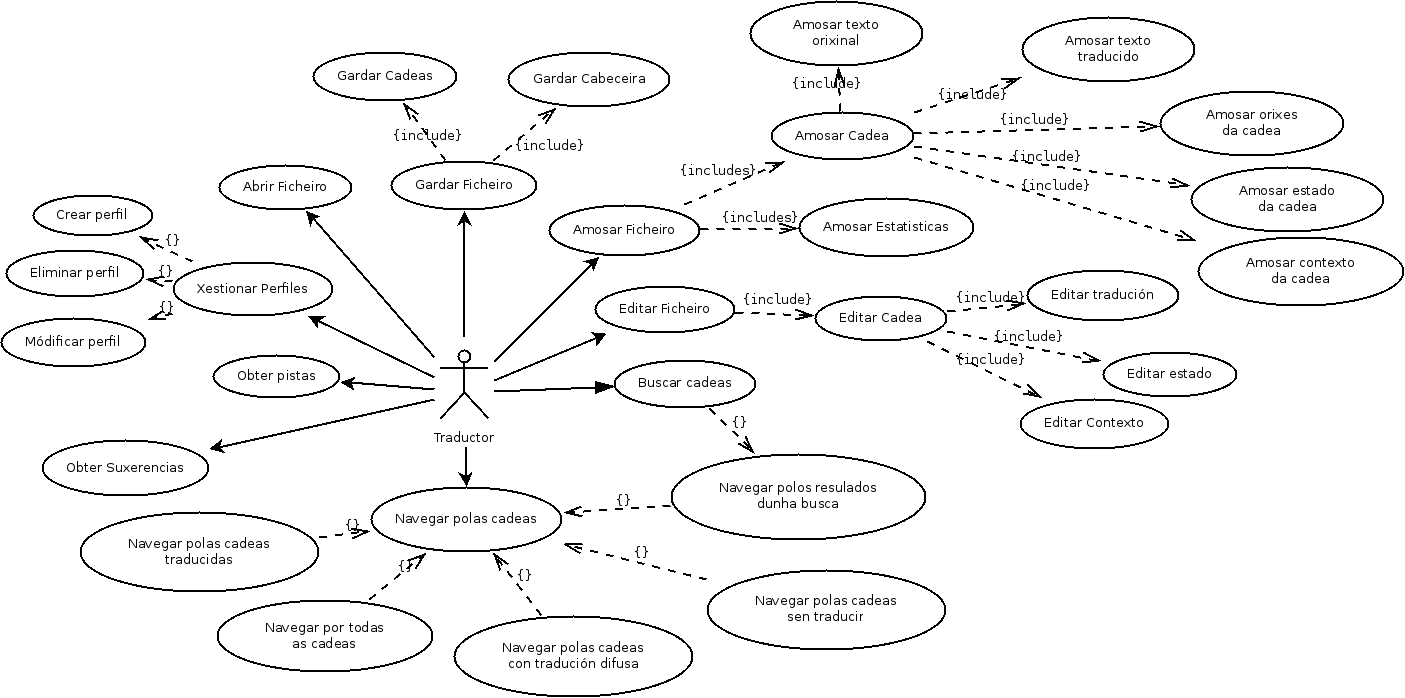
\includegraphics[width=0.9\textheight,angle=90]{img/casosdeuso.png}
    \caption{Diagrama UML de casos de uso do aplicativo}
    \label{fig:casosdeuso}
\end{figure}

%
% FIN DEL CAPÍTULO
%

        \chapter{Desarollo Iterativo}
        \chapter{Conclusións e Traballo futuro}

\section{Conclusións}

\section{Traballo Futuro}
Como calquera proxecto de software libre este programa é un proxecto inconcluso. Por unha parte moitos dos requisitos establecidos ao inicio do proxecto ou presentan deficiencias ou están elaborados con pouco detalle. Ademais aínda que neste proxecto a interface gráfica supuxo un esforzo importante, aínda hai algunhas partes que poden ser mellorables.

Por outro lado as contribución externas a este proxecto foron moi limitadas pois so contribuiron dúas persoas con cambios triviales. Para que un proxecto destas caracteristicas teña futuro é necesario crear unha comunidade arredor del. Polo que unha das liñas de traballo ten que ser buscar contribuidores para o proxecto e integralo dentro da infraestructura de GNOME.

Se falamos de liñas de traballo en canto a implementación de novas caracteristicas existen varias lineas de traballo moi interesantes:

\paragraph{Integración con Damned Lies.} Damned Lies é a plataforma oficial de GNOME para xestionar as traducións. Nela podense baixar os ficheiros para traducir, subir os ficheiros traducidos, revisar os mesmos, e ver as estatisticas xerais de tradución para cada linguaxe. Sería realmente útil que todas estas tarefas se puidesen facer dende GNOMECAT. Para isto non so bastaría con implementar novas vistas en GNOMECAT senón tamén a creación dunha API pública para a plataforma web Damned Lies que está escrita en Python empregando o framework Django.

\paragraph{Glosario.} Implementación dun glosario de termos na interface de edición de GNOMECAT. Este glosario debería permitir importar e exportar diversas bases de datos tanto online como offline.

\paragraph{Previsualización das traducións.} Como xa se comentou anteriormente esta é unha caracteristica moi interesante para unha ferramenta CAT pois permite que os traductores vexan como pode quedar a tradución no programa final. Aínda que existen varias alternativas para implementar esta funcionalidade semella que a máis axeitada para tecnoloxías GNOME é empregar o motor de renderizado Glade como se fixo na aplicación web Deckard.


  % INCLUIMOS LOS APÉNDICES...
        \appendix
        \chapter{Escoller a licencia do programa}

A hora de escoller unha licencia para o novo programa temos que ter en conta as licencias das bibliotecas empregadas no noso programa. Na siguente lista podense ver as bibliotecas empregadas para o programa así como a licencia de cada unha delas.

\begin{itemize}
  \item \textbf{GLib} GNU Lesser General Public License v2.1
  \item \textbf{GTK+} GNU Lesser General Public License v2.1
  \item \textbf{LibGee}  GNU Lesser General Public License v2.1
  \item \textbf{LibPeas} GNU Lesser General Public License v2.1
  \item \textbf{GettextPo} GNU General Public License v2
  \item \textbf{GTKSourceView} GNU Lesser General Public License v2.1
  \item \textbf{JSON-GLib} GNU Lesser General Public License v2.1
\end{itemize}

Como podemos ver excepto a biblioteca GettextPO, que emprega unha licencia GNU GPLv2, o resto de bibliotecas empregadas usan unha licencia GNU LGPL v2.1. A licencia GNU Lesser GPL permite empregar calquera licencia en productos derivados. Por outra parte a licencia GNU GPL v.2 obliga a empregar a licencia GNU GPL v2 ou versións posteriores da mesma licencia.

No noso caso eleximos a licencia GNU General Public Licence v3 que é unha versión máis actualizada da licencia para programas de GNU. No seguinte apéndice podese ver o texto completo desta licecia.


        \section{Licencia GPLv3}
\begin{center}
{\parindent 0in

Copyright \copyright\  2007 Free Software Foundation, Inc. \texttt{http://fsf.org/}

\bigskip
Everyone is permitted to copy and distribute verbatim copies of this

license document, but changing it is not allowed.}

\end{center}

\begin{center}
{\Large \sc Preamble}
\end{center}
The GNU General Public License is a free, copyleft license for
software and other kinds of works.

The licenses for most software and other practical works are designed
to take away your freedom to share and change the works.  By contrast,
the GNU General Public License is intended to guarantee your freedom to
share and change all versions of a program--to make sure it remains free
software for all its users.  We, the Free Software Foundation, use the
GNU General Public License for most of our software; it applies also to
any other work released this way by its authors.  You can apply it to
your programs, too.

When we speak of free software, we are referring to freedom, not
price.  Our General Public Licenses are designed to make sure that you
have the freedom to distribute copies of free software (and charge for
them if you wish), that you receive source code or can get it if you
want it, that you can change the software or use pieces of it in new
free programs, and that you know you can do these things.

To protect your rights, we need to prevent others from denying you
these rights or asking you to surrender the rights.  Therefore, you have
certain responsibilities if you distribute copies of the software, or if
you modify it: responsibilities to respect the freedom of others.

For example, if you distribute copies of such a program, whether
gratis or for a fee, you must pass on to the recipients the same
freedoms that you received.  You must make sure that they, too, receive
or can get the source code.  And you must show them these terms so they
know their rights.

Developers that use the GNU GPL protect your rights with two steps:
(1) assert copyright on the software, and (2) offer you this License
giving you legal permission to copy, distribute and/or modify it.

For the developers' and authors' protection, the GPL clearly explains
that there is no warranty for this free software.  For both users' and
authors' sake, the GPL requires that modified versions be marked as
changed, so that their problems will not be attributed erroneously to
authors of previous versions.

Some devices are designed to deny users access to install or run
modified versions of the software inside them, although the manufacturer
can do so.  This is fundamentally incompatible with the aim of
protecting users' freedom to change the software.  The systematic
pattern of such abuse occurs in the area of products for individuals to
use, which is precisely where it is most unacceptable.  Therefore, we
have designed this version of the GPL to prohibit the practice for those
products.  If such problems arise substantially in other domains, we
stand ready to extend this provision to those domains in future versions
of the GPL, as needed to protect the freedom of users.

Finally, every program is threatened constantly by software patents.
States should not allow patents to restrict development and use of
software on general-purpose computers, but in those that do, we wish to
avoid the special danger that patents applied to a free program could
make it effectively proprietary.  To prevent this, the GPL assures that
patents cannot be used to render the program non-free.

The precise terms and conditions for copying, distribution and
modification follow.

\begin{center}
{\Large \sc Terms and Conditions}
\end{center}


\begin{enumerate}

\addtocounter{enumi}{-1}

\item Definitions.

``This License'' refers to version 3 of the GNU General Public License.

``Copyright'' also means copyright-like laws that apply to other kinds of
works, such as semiconductor masks.

``The Program'' refers to any copyrightable work licensed under this
License.  Each licensee is addressed as ``you''.  ``Licensees'' and
``recipients'' may be individuals or organizations.

To ``modify'' a work means to copy from or adapt all or part of the work
in a fashion requiring copyright permission, other than the making of an
exact copy.  The resulting work is called a ``modified version'' of the
earlier work or a work ``based on'' the earlier work.

A ``covered work'' means either the unmodified Program or a work based
on the Program.

To ``propagate'' a work means to do anything with it that, without
permission, would make you directly or secondarily liable for
infringement under applicable copyright law, except executing it on a
computer or modifying a private copy.  Propagation includes copying,
distribution (with or without modification), making available to the
public, and in some countries other activities as well.

To ``convey'' a work means any kind of propagation that enables other
parties to make or receive copies.  Mere interaction with a user through
a computer network, with no transfer of a copy, is not conveying.

An interactive user interface displays ``Appropriate Legal Notices''
to the extent that it includes a convenient and prominently visible
feature that (1) displays an appropriate copyright notice, and (2)
tells the user that there is no warranty for the work (except to the
extent that warranties are provided), that licensees may convey the
work under this License, and how to view a copy of this License.  If
the interface presents a list of user commands or options, such as a
menu, a prominent item in the list meets this criterion.

\item Source Code.

The ``source code'' for a work means the preferred form of the work
for making modifications to it.  ``Object code'' means any non-source
form of a work.

A ``Standard Interface'' means an interface that either is an official
standard defined by a recognized standards body, or, in the case of
interfaces specified for a particular programming language, one that
is widely used among developers working in that language.

The ``System Libraries'' of an executable work include anything, other
than the work as a whole, that (a) is included in the normal form of
packaging a Major Component, but which is not part of that Major
Component, and (b) serves only to enable use of the work with that
Major Component, or to implement a Standard Interface for which an
implementation is available to the public in source code form.  A
``Major Component'', in this context, means a major essential component
(kernel, window system, and so on) of the specific operating system
(if any) on which the executable work runs, or a compiler used to
produce the work, or an object code interpreter used to run it.

The ``Corresponding Source'' for a work in object code form means all
the source code needed to generate, install, and (for an executable
work) run the object code and to modify the work, including scripts to
control those activities.  However, it does not include the work's
System Libraries, or general-purpose tools or generally available free
programs which are used unmodified in performing those activities but
which are not part of the work.  For example, Corresponding Source
includes interface definition files associated with source files for
the work, and the source code for shared libraries and dynamically
linked subprograms that the work is specifically designed to require,
such as by intimate data communication or control flow between those
subprograms and other parts of the work.

The Corresponding Source need not include anything that users
can regenerate automatically from other parts of the Corresponding
Source.

The Corresponding Source for a work in source code form is that
same work.

\item Basic Permissions.

All rights granted under this License are granted for the term of
copyright on the Program, and are irrevocable provided the stated
conditions are met.  This License explicitly affirms your unlimited
permission to run the unmodified Program.  The output from running a
covered work is covered by this License only if the output, given its
content, constitutes a covered work.  This License acknowledges your
rights of fair use or other equivalent, as provided by copyright law.

You may make, run and propagate covered works that you do not
convey, without conditions so long as your license otherwise remains
in force.  You may convey covered works to others for the sole purpose
of having them make modifications exclusively for you, or provide you
with facilities for running those works, provided that you comply with
the terms of this License in conveying all material for which you do
not control copyright.  Those thus making or running the covered works
for you must do so exclusively on your behalf, under your direction
and control, on terms that prohibit them from making any copies of
your copyrighted material outside their relationship with you.

Conveying under any other circumstances is permitted solely under
the conditions stated below.  Sublicensing is not allowed; section 10
makes it unnecessary.

\item Protecting Users' Legal Rights From Anti-Circumvention Law.

No covered work shall be deemed part of an effective technological
measure under any applicable law fulfilling obligations under article
11 of the WIPO copyright treaty adopted on 20 December 1996, or
similar laws prohibiting or restricting circumvention of such
measures.

When you convey a covered work, you waive any legal power to forbid
circumvention of technological measures to the extent such circumvention
is effected by exercising rights under this License with respect to
the covered work, and you disclaim any intention to limit operation or
modification of the work as a means of enforcing, against the work's
users, your or third parties' legal rights to forbid circumvention of
technological measures.

\item Conveying Verbatim Copies.

You may convey verbatim copies of the Program's source code as you
receive it, in any medium, provided that you conspicuously and
appropriately publish on each copy an appropriate copyright notice;
keep intact all notices stating that this License and any
non-permissive terms added in accord with section 7 apply to the code;
keep intact all notices of the absence of any warranty; and give all
recipients a copy of this License along with the Program.

You may charge any price or no price for each copy that you convey,
and you may offer support or warranty protection for a fee.

\item Conveying Modified Source Versions.

You may convey a work based on the Program, or the modifications to
produce it from the Program, in the form of source code under the
terms of section 4, provided that you also meet all of these conditions:
  \begin{enumerate}
  \item The work must carry prominent notices stating that you modified
  it, and giving a relevant date.

  \item The work must carry prominent notices stating that it is
  released under this License and any conditions added under section
  7.  This requirement modifies the requirement in section 4 to
  ``keep intact all notices''.

  \item You must license the entire work, as a whole, under this
  License to anyone who comes into possession of a copy.  This
  License will therefore apply, along with any applicable section 7
  additional terms, to the whole of the work, and all its parts,
  regardless of how they are packaged.  This License gives no
  permission to license the work in any other way, but it does not
  invalidate such permission if you have separately received it.

  \item If the work has interactive user interfaces, each must display
  Appropriate Legal Notices; however, if the Program has interactive
  interfaces that do not display Appropriate Legal Notices, your
  work need not make them do so.
\end{enumerate}
A compilation of a covered work with other separate and independent
works, which are not by their nature extensions of the covered work,
and which are not combined with it such as to form a larger program,
in or on a volume of a storage or distribution medium, is called an
``aggregate'' if the compilation and its resulting copyright are not
used to limit the access or legal rights of the compilation's users
beyond what the individual works permit.  Inclusion of a covered work
in an aggregate does not cause this License to apply to the other
parts of the aggregate.

\item Conveying Non-Source Forms.

You may convey a covered work in object code form under the terms
of sections 4 and 5, provided that you also convey the
machine-readable Corresponding Source under the terms of this License,
in one of these ways:
  \begin{enumerate}
  \item Convey the object code in, or embodied in, a physical product
  (including a physical distribution medium), accompanied by the
  Corresponding Source fixed on a durable physical medium
  customarily used for software interchange.

  \item Convey the object code in, or embodied in, a physical product
  (including a physical distribution medium), accompanied by a
  written offer, valid for at least three years and valid for as
  long as you offer spare parts or customer support for that product
  model, to give anyone who possesses the object code either (1) a
  copy of the Corresponding Source for all the software in the
  product that is covered by this License, on a durable physical
  medium customarily used for software interchange, for a price no
  more than your reasonable cost of physically performing this
  conveying of source, or (2) access to copy the
  Corresponding Source from a network server at no charge.

  \item Convey individual copies of the object code with a copy of the
  written offer to provide the Corresponding Source.  This
  alternative is allowed only occasionally and noncommercially, and
  only if you received the object code with such an offer, in accord
  with subsection 6b.

  \item Convey the object code by offering access from a designated
  place (gratis or for a charge), and offer equivalent access to the
  Corresponding Source in the same way through the same place at no
  further charge.  You need not require recipients to copy the
  Corresponding Source along with the object code.  If the place to
  copy the object code is a network server, the Corresponding Source
  may be on a different server (operated by you or a third party)
  that supports equivalent copying facilities, provided you maintain
  clear directions next to the object code saying where to find the
  Corresponding Source.  Regardless of what server hosts the
  Corresponding Source, you remain obligated to ensure that it is
  available for as long as needed to satisfy these requirements.

  \item Convey the object code using peer-to-peer transmission, provided
  you inform other peers where the object code and Corresponding
  Source of the work are being offered to the general public at no
  charge under subsection 6d.
  \end{enumerate}

A separable portion of the object code, whose source code is excluded
from the Corresponding Source as a System Library, need not be
included in conveying the object code work.

A ``User Product'' is either (1) a ``consumer product'', which means any
tangible personal property which is normally used for personal, family,
or household purposes, or (2) anything designed or sold for incorporation
into a dwelling.  In determining whether a product is a consumer product,
doubtful cases shall be resolved in favor of coverage.  For a particular
product received by a particular user, ``normally used'' refers to a
typical or common use of that class of product, regardless of the status
of the particular user or of the way in which the particular user
actually uses, or expects or is expected to use, the product.  A product
is a consumer product regardless of whether the product has substantial
commercial, industrial or non-consumer uses, unless such uses represent
the only significant mode of use of the product.

``Installation Information'' for a User Product means any methods,
procedures, authorization keys, or other information required to install
and execute modified versions of a covered work in that User Product from
a modified version of its Corresponding Source.  The information must
suffice to ensure that the continued functioning of the modified object
code is in no case prevented or interfered with solely because
modification has been made.

If you convey an object code work under this section in, or with, or
specifically for use in, a User Product, and the conveying occurs as
part of a transaction in which the right of possession and use of the
User Product is transferred to the recipient in perpetuity or for a
fixed term (regardless of how the transaction is characterized), the
Corresponding Source conveyed under this section must be accompanied
by the Installation Information.  But this requirement does not apply
if neither you nor any third party retains the ability to install
modified object code on the User Product (for example, the work has
been installed in ROM).

The requirement to provide Installation Information does not include a
requirement to continue to provide support service, warranty, or updates
for a work that has been modified or installed by the recipient, or for
the User Product in which it has been modified or installed.  Access to a
network may be denied when the modification itself materially and
adversely affects the operation of the network or violates the rules and
protocols for communication across the network.

Corresponding Source conveyed, and Installation Information provided,
in accord with this section must be in a format that is publicly
documented (and with an implementation available to the public in
source code form), and must require no special password or key for
unpacking, reading or copying.

\item Additional Terms.

``Additional permissions'' are terms that supplement the terms of this
License by making exceptions from one or more of its conditions.
Additional permissions that are applicable to the entire Program shall
be treated as though they were included in this License, to the extent
that they are valid under applicable law.  If additional permissions
apply only to part of the Program, that part may be used separately
under those permissions, but the entire Program remains governed by
this License without regard to the additional permissions.

When you convey a copy of a covered work, you may at your option
remove any additional permissions from that copy, or from any part of
it.  (Additional permissions may be written to require their own
removal in certain cases when you modify the work.)  You may place
additional permissions on material, added by you to a covered work,
for which you have or can give appropriate copyright permission.

Notwithstanding any other provision of this License, for material you
add to a covered work, you may (if authorized by the copyright holders of
that material) supplement the terms of this License with terms:
  \begin{enumerate}
  \item Disclaiming warranty or limiting liability differently from the
  terms of sections 15 and 16 of this License; or

  \item Requiring preservation of specified reasonable legal notices or
  author attributions in that material or in the Appropriate Legal
  Notices displayed by works containing it; or

  \item Prohibiting misrepresentation of the origin of that material, or
  requiring that modified versions of such material be marked in
  reasonable ways as different from the original version; or

  \item Limiting the use for publicity purposes of names of licensors or
  authors of the material; or

  \item Declining to grant rights under trademark law for use of some
  trade names, trademarks, or service marks; or

  \item Requiring indemnification of licensors and authors of that
  material by anyone who conveys the material (or modified versions of
  it) with contractual assumptions of liability to the recipient, for
  any liability that these contractual assumptions directly impose on
  those licensors and authors.
  \end{enumerate}

All other non-permissive additional terms are considered ``further
restrictions'' within the meaning of section 10.  If the Program as you
received it, or any part of it, contains a notice stating that it is
governed by this License along with a term that is a further
restriction, you may remove that term.  If a license document contains
a further restriction but permits relicensing or conveying under this
License, you may add to a covered work material governed by the terms
of that license document, provided that the further restriction does
not survive such relicensing or conveying.

If you add terms to a covered work in accord with this section, you
must place, in the relevant source files, a statement of the
additional terms that apply to those files, or a notice indicating
where to find the applicable terms.

Additional terms, permissive or non-permissive, may be stated in the
form of a separately written license, or stated as exceptions;
the above requirements apply either way.

\item Termination.

You may not propagate or modify a covered work except as expressly
provided under this License.  Any attempt otherwise to propagate or
modify it is void, and will automatically terminate your rights under
this License (including any patent licenses granted under the third
paragraph of section 11).

However, if you cease all violation of this License, then your
license from a particular copyright holder is reinstated (a)
provisionally, unless and until the copyright holder explicitly and
finally terminates your license, and (b) permanently, if the copyright
holder fails to notify you of the violation by some reasonable means
prior to 60 days after the cessation.

Moreover, your license from a particular copyright holder is
reinstated permanently if the copyright holder notifies you of the
violation by some reasonable means, this is the first time you have
received notice of violation of this License (for any work) from that
copyright holder, and you cure the violation prior to 30 days after
your receipt of the notice.

Termination of your rights under this section does not terminate the
licenses of parties who have received copies or rights from you under
this License.  If your rights have been terminated and not permanently
reinstated, you do not qualify to receive new licenses for the same
material under section 10.

\item Acceptance Not Required for Having Copies.

You are not required to accept this License in order to receive or
run a copy of the Program.  Ancillary propagation of a covered work
occurring solely as a consequence of using peer-to-peer transmission
to receive a copy likewise does not require acceptance.  However,
nothing other than this License grants you permission to propagate or
modify any covered work.  These actions infringe copyright if you do
not accept this License.  Therefore, by modifying or propagating a
covered work, you indicate your acceptance of this License to do so.

\item Automatic Licensing of Downstream Recipients.

Each time you convey a covered work, the recipient automatically
receives a license from the original licensors, to run, modify and
propagate that work, subject to this License.  You are not responsible
for enforcing compliance by third parties with this License.

An ``entity transaction'' is a transaction transferring control of an
organization, or substantially all assets of one, or subdividing an
organization, or merging organizations.  If propagation of a covered
work results from an entity transaction, each party to that
transaction who receives a copy of the work also receives whatever
licenses to the work the party's predecessor in interest had or could
give under the previous paragraph, plus a right to possession of the
Corresponding Source of the work from the predecessor in interest, if
the predecessor has it or can get it with reasonable efforts.

You may not impose any further restrictions on the exercise of the
rights granted or affirmed under this License.  For example, you may
not impose a license fee, royalty, or other charge for exercise of
rights granted under this License, and you may not initiate litigation
(including a cross-claim or counterclaim in a lawsuit) alleging that
any patent claim is infringed by making, using, selling, offering for
sale, or importing the Program or any portion of it.

\item Patents.

A ``contributor'' is a copyright holder who authorizes use under this
License of the Program or a work on which the Program is based.  The
work thus licensed is called the contributor's ``contributor version''.

A contributor's ``essential patent claims'' are all patent claims
owned or controlled by the contributor, whether already acquired or
hereafter acquired, that would be infringed by some manner, permitted
by this License, of making, using, or selling its contributor version,
but do not include claims that would be infringed only as a
consequence of further modification of the contributor version.  For
purposes of this definition, ``control'' includes the right to grant
patent sublicenses in a manner consistent with the requirements of
this License.

Each contributor grants you a non-exclusive, worldwide, royalty-free
patent license under the contributor's essential patent claims, to
make, use, sell, offer for sale, import and otherwise run, modify and
propagate the contents of its contributor version.

In the following three paragraphs, a ``patent license'' is any express
agreement or commitment, however denominated, not to enforce a patent
(such as an express permission to practice a patent or covenant not to
sue for patent infringement).  To ``grant'' such a patent license to a
party means to make such an agreement or commitment not to enforce a
patent against the party.

If you convey a covered work, knowingly relying on a patent license,
and the Corresponding Source of the work is not available for anyone
to copy, free of charge and under the terms of this License, through a
publicly available network server or other readily accessible means,
then you must either (1) cause the Corresponding Source to be so
available, or (2) arrange to deprive yourself of the benefit of the
patent license for this particular work, or (3) arrange, in a manner
consistent with the requirements of this License, to extend the patent
license to downstream recipients.  ``Knowingly relying'' means you have
actual knowledge that, but for the patent license, your conveying the
covered work in a country, or your recipient's use of the covered work
in a country, would infringe one or more identifiable patents in that
country that you have reason to believe are valid.

If, pursuant to or in connection with a single transaction or
arrangement, you convey, or propagate by procuring conveyance of, a
covered work, and grant a patent license to some of the parties
receiving the covered work authorizing them to use, propagate, modify
or convey a specific copy of the covered work, then the patent license
you grant is automatically extended to all recipients of the covered
work and works based on it.

A patent license is ``discriminatory'' if it does not include within
the scope of its coverage, prohibits the exercise of, or is
conditioned on the non-exercise of one or more of the rights that are
specifically granted under this License.  You may not convey a covered
work if you are a party to an arrangement with a third party that is
in the business of distributing software, under which you make payment
to the third party based on the extent of your activity of conveying
the work, and under which the third party grants, to any of the
parties who would receive the covered work from you, a discriminatory
patent license (a) in connection with copies of the covered work
conveyed by you (or copies made from those copies), or (b) primarily
for and in connection with specific products or compilations that
contain the covered work, unless you entered into that arrangement,
or that patent license was granted, prior to 28 March 2007.

Nothing in this License shall be construed as excluding or limiting
any implied license or other defenses to infringement that may
otherwise be available to you under applicable patent law.

\item No Surrender of Others' Freedom.

If conditions are imposed on you (whether by court order, agreement or
otherwise) that contradict the conditions of this License, they do not
excuse you from the conditions of this License.  If you cannot convey a
covered work so as to satisfy simultaneously your obligations under this
License and any other pertinent obligations, then as a consequence you may
not convey it at all.  For example, if you agree to terms that obligate you
to collect a royalty for further conveying from those to whom you convey
the Program, the only way you could satisfy both those terms and this
License would be to refrain entirely from conveying the Program.

\item Use with the GNU Affero General Public License.

Notwithstanding any other provision of this License, you have
permission to link or combine any covered work with a work licensed
under version 3 of the GNU Affero General Public License into a single
combined work, and to convey the resulting work.  The terms of this
License will continue to apply to the part which is the covered work,
but the special requirements of the GNU Affero General Public License,
section 13, concerning interaction through a network will apply to the
combination as such.

\item Revised Versions of this License.

The Free Software Foundation may publish revised and/or new versions of
the GNU General Public License from time to time.  Such new versions will
be similar in spirit to the present version, but may differ in detail to
address new problems or concerns.

Each version is given a distinguishing version number.  If the
Program specifies that a certain numbered version of the GNU General
Public License ``or any later version'' applies to it, you have the
option of following the terms and conditions either of that numbered
version or of any later version published by the Free Software
Foundation.  If the Program does not specify a version number of the
GNU General Public License, you may choose any version ever published
by the Free Software Foundation.

If the Program specifies that a proxy can decide which future
versions of the GNU General Public License can be used, that proxy's
public statement of acceptance of a version permanently authorizes you
to choose that version for the Program.

Later license versions may give you additional or different
permissions.  However, no additional obligations are imposed on any
author or copyright holder as a result of your choosing to follow a
later version.

\item Disclaimer of Warranty.

\begin{sloppypar}
 THERE IS NO WARRANTY FOR THE PROGRAM, TO THE EXTENT PERMITTED BY
 APPLICABLE LAW.  EXCEPT WHEN OTHERWISE STATED IN WRITING THE
 COPYRIGHT HOLDERS AND/OR OTHER PARTIES PROVIDE THE PROGRAM ``AS IS''
 WITHOUT WARRANTY OF ANY KIND, EITHER EXPRESSED OR IMPLIED,
 INCLUDING, BUT NOT LIMITED TO, THE IMPLIED WARRANTIES OF
 MERCHANTABILITY AND FITNESS FOR A PARTICULAR PURPOSE.  THE ENTIRE
 RISK AS TO THE QUALITY AND PERFORMANCE OF THE PROGRAM IS WITH YOU.
 SHOULD THE PROGRAM PROVE DEFECTIVE, YOU ASSUME THE COST OF ALL
 NECESSARY SERVICING, REPAIR OR CORRECTION.
\end{sloppypar}

\item Limitation of Liability.

 IN NO EVENT UNLESS REQUIRED BY APPLICABLE LAW OR AGREED TO IN
 WRITING WILL ANY COPYRIGHT HOLDER, OR ANY OTHER PARTY WHO MODIFIES
 AND/OR CONVEYS THE PROGRAM AS PERMITTED ABOVE, BE LIABLE TO YOU FOR
 DAMAGES, INCLUDING ANY GENERAL, SPECIAL, INCIDENTAL OR CONSEQUENTIAL
 DAMAGES ARISING OUT OF THE USE OR INABILITY TO USE THE PROGRAM
 (INCLUDING BUT NOT LIMITED TO LOSS OF DATA OR DATA BEING RENDERED
 INACCURATE OR LOSSES SUSTAINED BY YOU OR THIRD PARTIES OR A FAILURE
 OF THE PROGRAM TO OPERATE WITH ANY OTHER PROGRAMS), EVEN IF SUCH
 HOLDER OR OTHER PARTY HAS BEEN ADVISED OF THE POSSIBILITY OF SUCH
 DAMAGES.

\item Interpretation of Sections 15 and 16.

If the disclaimer of warranty and limitation of liability provided
above cannot be given local legal effect according to their terms,
reviewing courts shall apply local law that most closely approximates
an absolute waiver of all civil liability in connection with the
Program, unless a warranty or assumption of liability accompanies a
copy of the Program in return for a fee.

\begin{center}
{\Large\sc End of Terms and Conditions}

\bigskip
How to Apply These Terms to Your New Programs
\end{center}

If you develop a new program, and you want it to be of the greatest
possible use to the public, the best way to achieve this is to make it
free software which everyone can redistribute and change under these terms.

To do so, attach the following notices to the program.  It is safest
to attach them to the start of each source file to most effectively
state the exclusion of warranty; and each file should have at least
the ``copyright'' line and a pointer to where the full notice is found.

{\footnotesize
\begin{verbatim}
<one line to give the program's name and a brief idea of what it does.>

Copyright (C) <textyear>  <name of author>

This program is free software: you can redistribute it and/or modify
it under the terms of the GNU General Public License as published by
the Free Software Foundation, either version 3 of the License, or
(at your option) any later version.

This program is distributed in the hope that it will be useful,
but WITHOUT ANY WARRANTY; without even the implied warranty of
MERCHANTABILITY or FITNESS FOR A PARTICULAR PURPOSE.  See the
GNU General Public License for more details.

You should have received a copy of the GNU General Public License
along with this program.  If not, see <http://www.gnu.org/licenses/>.
\end{verbatim}
}

Also add information on how to contact you by electronic and paper mail.

If the program does terminal interaction, make it output a short
notice like this when it starts in an interactive mode:

{\footnotesize
\begin{verbatim}
<program>  Copyright (C) <year>  <name of author>

This program comes with ABSOLUTELY NO WARRANTY; for details type `show w'.
This is free software, and you are welcome to redistribute it
under certain conditions; type `show c' for details.
\end{verbatim}
}

The hypothetical commands {\tt show w} and {\tt show c} should show
the appropriate
parts of the General Public License.  Of course, your program's commands
might be different; for a GUI interface, you would use an ``about box''.

You should also get your employer (if you work as a programmer) or
school, if any, to sign a ``copyright disclaimer'' for the program, if
necessary.  For more information on this, and how to apply and follow
the GNU GPL, see \texttt{http://www.gnu.org/licenses/}.

The GNU General Public License does not permit incorporating your
program into proprietary programs.  If your program is a subroutine
library, you may consider it more useful to permit linking proprietary
applications with the library.  If this is what you want to do, use
the GNU Lesser General Public License instead of this License.  But
first, please read \texttt{http://www.gnu.org/philosophy/why-not-lgpl.html}.

\end{enumerate}

       %\include{pfc_appendix_020}


  % INCLUIMOS LA BIBLIOGRAFÍA...
        \nocite{*}  % Se usa para indicar en la bibliograf? las referencias no citadas.
        \bibliography{pfc_biblio}
        \bibliographystyle{plain}

\end{document}

